\documentclass[a4paper,12pt,twoside]{article}

%PACKAGES

\usepackage[T1]{fontenc}
\usepackage{lmodern}

\usepackage[utf8]{inputenc}
\usepackage[slovak]{babel}
\usepackage{comment}

\usepackage{array}

\usepackage{graphicx,amsmath,amssymb, amsthm, multicol}
\usepackage{pdfpages}
\usepackage{float}

\usepackage[nottoc]{tocbibind}
\usepackage{mathrsfs}
\usepackage{psfrag}
\usepackage[small,bf]{caption}
\usepackage{ifthen}
\usepackage{titlesec}
\usepackage{makecell}

\usepackage{xcolor}
\usepackage{listings}
\usepackage{enumitem}
\usepackage{longtable}

\usepackage[toc,page]{appendix}

\usepackage{url}
\urlstyle{rm}
\renewcommand\UrlFont{\color{black}}

\usepackage{pgfplots}
\pgfplotsset{compat=1.16}

\usepackage{tikz}
\usetikzlibrary{positioning,chains,fit,shapes,calc}

% \renewcommand{\familydefault}{\rmdefault}

\newtheorem{defin}{Definícia}[section]
\newtheorem{theorem}[defin]{Veta}
\newtheorem{prop}[defin]{Tvrdenie}
\newtheorem{lema}[defin]{Lema}
\newtheorem{cor}[defin]{Dôsledok}
\newtheorem{hypoteza}{Hypotéza}[section]
\newtheoremstyle{comment}{}{}{}{}{}{:}{ }{#1}
\theoremstyle{comment}
\newtheorem{dokaz}{Dôkaz}[section]
\newtheorem{com}{\textit{Poznámka}}

\usepackage{hyperref}                                     
\hypersetup{%  http://www.tug.org/applications/hyperref/
bookmarksnumbered,
pdfstartview={FitH},
linkcolor=black,
citecolor=black,
colorlinks=true,
pdfpagemode={None},
plainpages=false
}%

%%\usepackage{fullpage}
%%\setlength{\topmargin}{-0.5cm}
%%\setlength{\headheight}{0cm}
%%\setlength{\headsep}{0in}
\setlength{\textheight}{24cm}
\setlength{\textwidth}{15.5cm}
\addtolength{\voffset}{-1.2cm}
\addtolength{\hoffset}{-0.3cm}
%%\addtolength{\rightmargin}{-1cm}
\setlength{\parindent}{0.5cm}
\setlength{\parskip}{0in}
\linespread{1.5}

\setcounter{MaxMatrixCols}{20}

\titleformat{\paragraph}
{\normalfont\normalsize\bfseries}{\theparagraph}{1em}{}
\titlespacing*{\paragraph}
{0pt}{3.25ex plus 1ex minus .2ex}{1.5ex plus .2ex}

\begin{document}

  \thispagestyle{empty}
\begin{center}
{\large \bf UNIVERZITA KOMENSKÉHO V BRATISLAVE \\
FAKULTA MATEMATIKY, FYZIKY A INFORMATIKY}
\end{center}
%\begin{titlepage}
%    \rmfamily
%    \begin{center}
%      \LARGE\scshape
%      \theuniversity\\
%      \Large\upshape
%      \thefaculty\\
%      \large
%      \thedepartment
%    \end{center}
%

\vspace{2cm}
\begin{figure}[!h]
   \centering
     %
\includegraphics[width=3.5cm]{logoUK.jpg}
\end{figure}

\vspace{1cm}
\begin{center}
{\large \bf Predikcia bankrotu firiem v slovenskom prostredí \\
\vspace{3cm}
DIPLOMOVÁ PRÁCA}
\end{center}

\vfill
%
\begin{multicols}{2}
{\bf
\begin{flushleft} 2022 \end{flushleft}
\begin{flushright} Bc. Róbert Druska \end{flushright} 
}
\end{multicols}


  \newpage
\thispagestyle{empty}
\begin{center}
{\large UNIVERZITA KOMENSKÉHO V BRATISLAVE \\
FAKULTA MATEMATIKY, FYZIKY A INFORMATIKY}
\end{center}


\vspace{5cm}
\begin{center}
{\large \bf Predikcia úpadku slovenských firiem \\
\vspace{3cm}
DIPLOMOVÁ PRÁCA}
\end{center}

\vfill
\begin{flushleft}
\begin{tabular}{ll}
Študijný program: & Pravdepodobnosť a matematická štatistika \\
Študijný odbor: & Aplikovaná matematika \\
Školiace pracovisko: & Katedra aplikovanej matematiky a štatistiky \\
Vedúci práce: & doc. Mgr. Radoslav Harman, PhD. \\
\end{tabular}
\end{flushleft}

\vfill
%
\begin{multicols}{2}
\begin{flushleft} Bratislava 2022 \end{flushleft}
\begin{flushright} {\bf Bc. Róbert Druska} \end{flushright}
\end{multicols}



  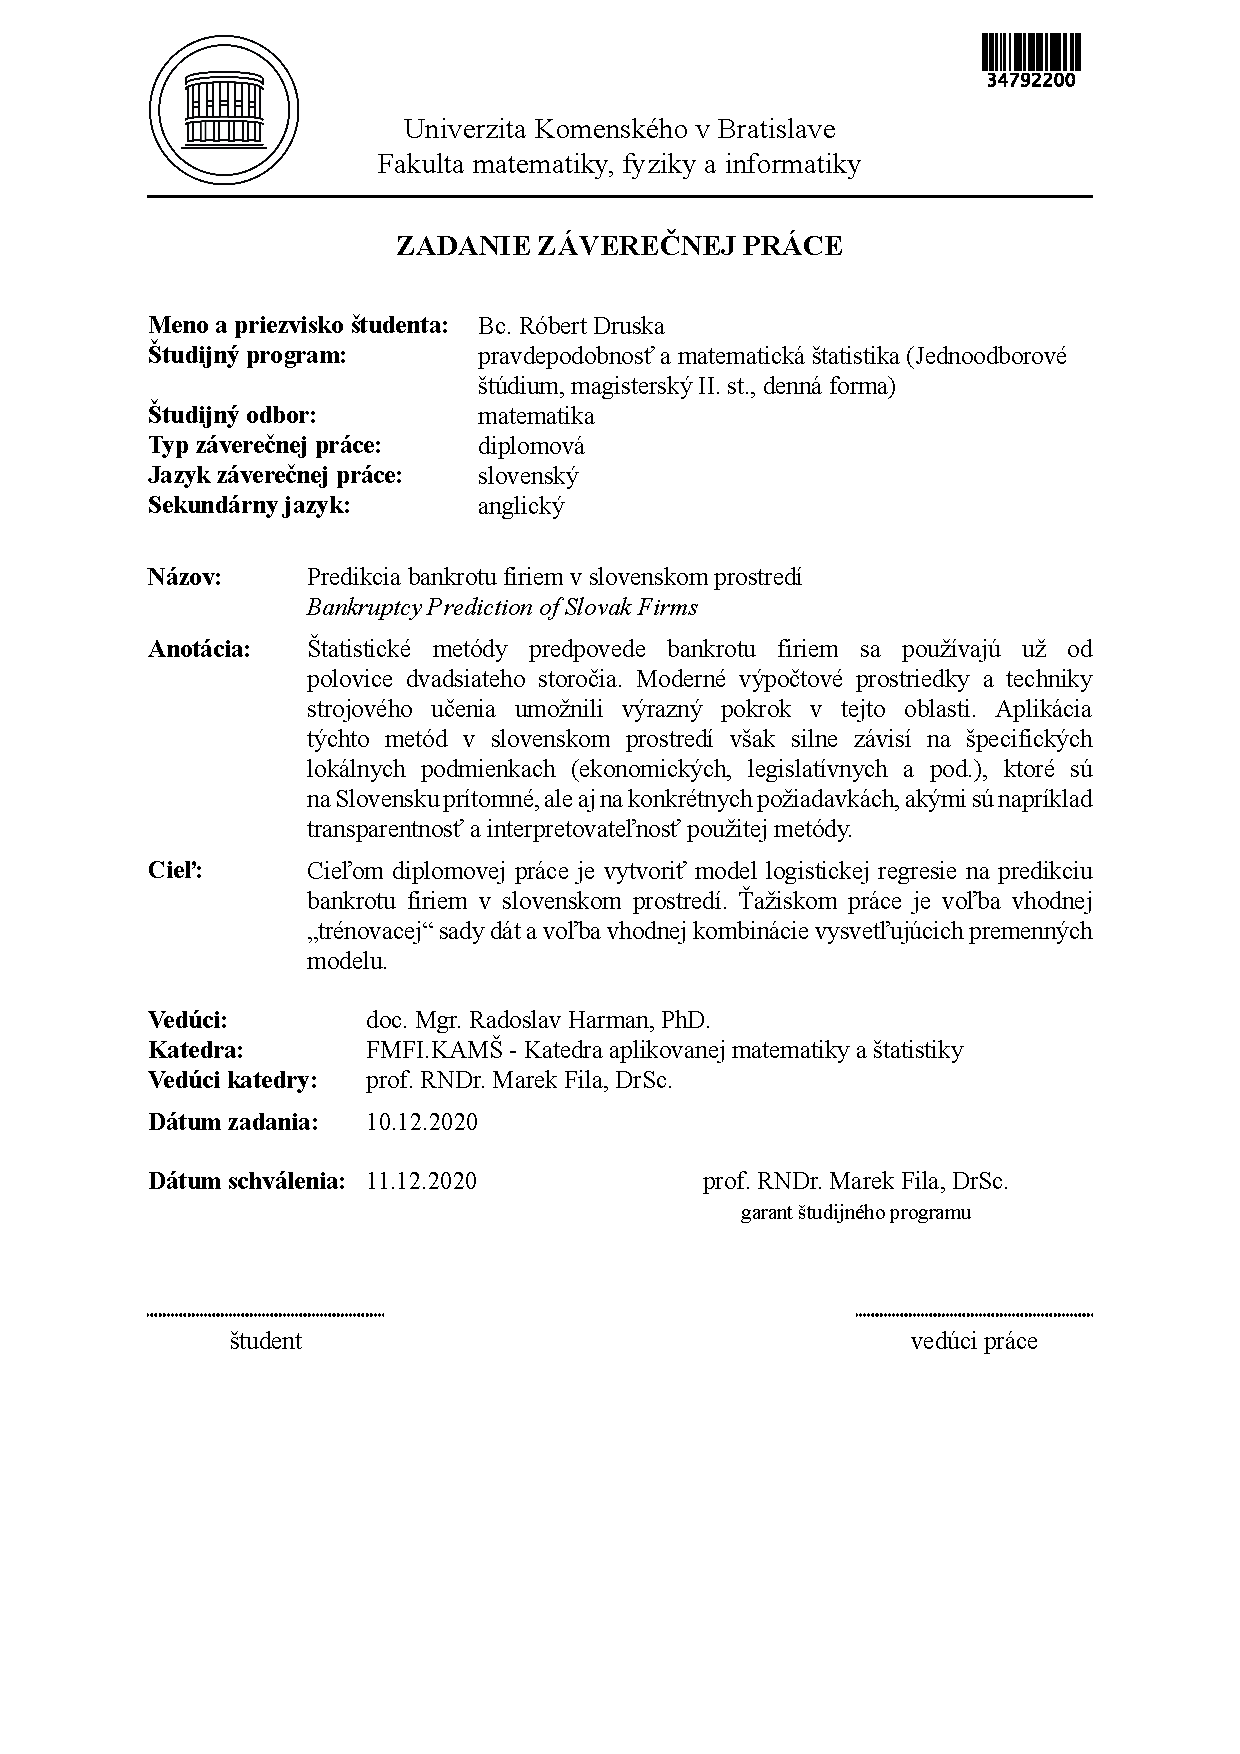
\includepdf[pages={1}, offset=25 -75]{zadanieRD.pdf}

  

\vglue0pt
\vfill
\thispagestyle{empty}
\paragraph{Poďakovanie}

Touto cestou by som sa chcel poďakovať svojmu školiteľovi, Radoslavovi Harmanovi, za jeho ochotu a množstvo dobrých a pravidelných rád pri písaní tejto práce.
Ďakujem tiež svojej kolegyni Monike Hrnčárovej za cenné analýzy predchádzajúce praktickým častiam práce, a svojej mame za gramatickú a štylistickú korektúru.
V neposlednom rade ďakujem svojim priateľom za oporu v posledných mesiacoch písania.


  \newpage
  \thispagestyle{empty}
\section*{Abstrakt}
DRUSKA, Róbert: Predikcia úpadku slovenských firiem [Diplomová práca],
Univerzita Komenského v Bratislave,
Fakulta matematiky, fyziky a informatiky,
Katedra aplikovanej matematiky a štatistiky,
školiteľ: doc. Mgr. Radoslav Harman, PhD.,
Bratislava, 2020, TODO s.

TODO Lorem ipsum dolor sit amet, consectetur adipiscing elit, sed do eiusmod tempor incididunt ut labore et dolore magna aliqua. Ut enim ad minim veniam, quis nostrud exercitation ullamco laboris nisi ut aliquip ex ea commodo consequat. Duis aute irure dolor in reprehenderit in voluptate velit esse cillum dolore eu fugiat nulla pariatur. Excepteur sint occaecat cupidatat non proident, sunt in culpa qui officia deserunt mollit anim id est laborum.

\begin{flushleft}
  \textbf{Kľúčové slová:} logistická regresia, TODO
\end{flushleft}

  \newpage
  \thispagestyle{empty}
\section*{Abstract}
DRUSKA, Róbert: Bankruptcy prediction [Master thesis],
Comenius University in Bratislava,
Faculty of Mathematics, Physics and Informatics,
Department of Applied Mathematics and Statistics,
supervisor: doc. Mgr. Radoslav Harman, PhD.,
Bratislava, 2020, TODO p.

TODO Lorem ipsum dolor sit amet, consectetur adipiscing elit, sed do eiusmod tempor incididunt ut labore et dolore magna aliqua. Ut enim ad minim veniam, quis nostrud exercitation ullamco laboris nisi ut aliquip ex ea commodo consequat. Duis aute irure dolor in reprehenderit in voluptate velit esse cillum dolore eu fugiat nulla pariatur. Excepteur sint occaecat cupidatat non proident, sunt in culpa qui officia deserunt mollit anim id est laborum.

\begin{flushleft}
  \textbf{Keywords:} logistic regression, TODO
\end{flushleft}
  \newpage \tableofcontents
  \setcounter{page}{7}
 % \newpage
 % \listoffigures
 % \newpage
 % \listoftables  
  \newpage

    \section*{Úvod}	          
    \markboth{ÚVOD}{ÚVOD}  
    \addcontentsline{toc}{section}{Úvod}
    
    Predikcia bankrotu firiem je predmetom akademického aj profesionálneho výskumu už po dlhé desaťročia.
Motivácia stojaca za hľadaním modelov na predikciu úpadku firiem je rôzna.
Prvé modely vytvorené na základe dát o verejne obchodovateľných spoločnostiach v USA
boli využívané pri analýzach predchádzajúcich nákupom akcií \cite{altman1968}.
Modely kreditného rizika našli veľké využitie v bankovníctve – banky a iné finančné inštitúcie disponujú internými modelmi,
ktorými vyhodnocujú finančnú kondíciu svojich klientov a ich hodnotenia využívajú napr. pri stanovovaní úrokových sadzieb.
Takisto aj súkromné spoločnosti a živnostníci môžu využiť modely kreditného rizika pri bežnom vykonávaní svojej podnikateľskej praxe.

V prvých dvoch kapitolách sa oboznamujeme s problematikou bankrotu na Slovenku a predstavíme si dva známe modely kreditného rizika – Altmanovo Z-skóre a český index IN05.
Tretia kapitola je teoretickou predprípravou k metodike,
ktorú sme v práci použili na modelovanie predikcie bankrotu v slovenskom prostredí.
Oboznámime sa v nej s logistickou regresiou a tiež s metódou \emph{BACE}, ktorá slúži na výber vhodnej kombinácie parametrov do modelu.
V štvrtej kapitole sa bližšie venujeme metodike praktickej časti práce.

V piatej kapitole dôkladne opíšeme proces vytvorenia modelov predikcie bankrotu
od popisu dát cez technické detaily modelovania až po porovnanie nami vytvorených modelov s Altmanovým Z-skóre a indexom IN05
aj medzi sebou navzájom. Posledná, šiesta kapitola obsahuje diskusiu o interpretácii výstupov bankrotových modelov. 

    \newpage
    \section{Bankrot na Slovensku}
\label{bankruptcy}

Cieľom tejto práce je vytvoriť model na predikciu úpadku firiem na základe jej finančných údajov.
Pre účely modelovania si na začiatok zadefinujme, čo budeme rozumieť pod pojmom úpadok.
Problematikou bankrotu právnických a fyzických osôb na Slovensku sa venuje najmä zákon 7/2005 Z. z. o konkurze a reštrukuturalizácii \cite{zbierkazakonov},
ktorý definuje úpadok nasledovne.

\bigskip
\textit{(1)
Dlžník je v úpadku, ak je platobne neschopný alebo predlžený. Ak dlžník podá návrh na vyhlásenie konkurzu, predpokladá sa, že je v úpadku.}

\textit{(2)
Právnická osoba je platobne neschopná, ak nie je schopná plniť 30 dní po lehote splatnosti aspoň dva peňažné záväzky viac ako jednému veriteľovi. […]}

\textit{(3)
Predlžený je ten, kto je povinný viesť účtovníctvo podľa osobitného predpisu, má viac ako jedného veriteľa a hodnota jeho záväzkov presahuje hodnotu jeho majetku. […]}
\bigskip

Keď je právnická osoba v úpadku, je potrebné vyhlásiť konkurz alebo reštrukturalizáciu.
Konkurzné a reštrukturalizačné konania schvaľuje súd, vďaka čomu poznáme presný dátum ich začiatku, čo sa nám zíde pri modelovaní.

Konkurz znamená speňaženie majetkovej podstaty dlžníka a pomerné uspokojenie jeho veriteľov z tohto majetku.
Konkurz má charakter likvidačného konania a jeho výsledkom je zrušenie a zánik podniku.
V bežnej praxi ide o zdĺhavý proces, ktorý môže trvať aj niekoľko rokov.

Na rozdiel od konkurzu reštrukturalizácia nemá likvidačný charakter a je možné vyhlásiť ju už v čase hroziaceho úpadku.
Cieľom reštrukturalizácie je zachovanie podniku alebo jeho časti a postupné uspokojenie veriteľov spôsobom dohodnutým v reštrukturalizačnom pláne.
Uspokojenie pohľadávok býva v praxi rýchlejšie ako pri konkurze.
V prípade, že reštrukturalizácia bude úspešná, právnická osoba može naďalej pokračovať v podnikateľskej činnosti,
avšak predpokladom jej úspechu je to, že pohľadávky veriteľov sa budú počas ďalšieho fungovania podniku uspokojovať vo vyššej miere ako v prípade konkurzu.

Spoločným znakom konkurzu a reštrukturalizácie je skutočnosť, že dlžník sa nachádza v krízovej ekonomickej situácii.
Pre účely tejto práce budeme \emph{bankrotom} rozumieť začiatok konkurzného alebo reštrukturalizačného konania.

\subsection{Bankrot - vzácna udalosť}

Úpadok alebo bankrot možno považovať v rámci populácie aktívnych firiem za vzácnu udalosť.
Databáza \emph{FinStat}, ktorej dáta budeme využívať v tejto práci, eviduje celkovo 6946 prípadov konkurzného alebo reštrukturalizačného konania za obdobie existencie samostatnej Slovenskej republiky.
Ako uvidíme, nie každé z týchto konaní sa hodí na modelovanie, či už kvôli nedostatku dostupných dát alebo inej príčiny.

Napríklad, z počtu 6946 firiem v úpadku len pre 3730 firiem poznáme presný dátum začiatku konkurzného alebo reštrukturalizačného konania.
Dátum začiatku konania nepoznáme zväčša pre staršie firmy, ktoré zanikli pred rokom 2010, a pre ktoré by sme v mnohých prípadoch aj tak nemali dostatok dát pre úspešné zahrnutie do modelu.

V tabuľke uvádzame počet konkurzov a reštrukturalizácií a počet aktívnych firiem od roku 2011 po rok 2020.

\begin{center}
    \begin{tabular}{ |c|c|c|c|p{3cm}|p{3cm}| }
        \hline
        Rok & Konkurzy & Reštrukturalizácie & Spolu & Celkový počet aktívnych firiem & Proporcia firiem v úpadku \\
        \hline
        2011 & 282 & 21 & 303 & TODO & TODO \\
        \hline
        2012 & 296 & 36 & 332 & & \\
        \hline
        2013 & 318 & 49 & 367 & & \\
        \hline
        2014 & 329 & 56 & 385 & & \\
        \hline
        2015 & 325 & 49 & 374 & & \\
        \hline
        2016 & 222 & 35 & 257 & & \\
        \hline
        2017 & 215 & 22 & 237 & & \\
        \hline
        2018 & 256 & 6 & 262 & & \\
        \hline
        2019 & 254 & 8 & 262 & & \\
        % pozn: v roku 2019 mala jedna firma konanie s kategoriou "ine", ide o firmu s ico 36595098 ... po rucnej kontrole som ju zaradil medzi restrukturalizacie
        \hline
        2020 & 185 & 19 & 204 & & \\
        \hline
    \end{tabular}
\end{center}
\bigskip

Ako vidíme, počet firiem v úpadku sa každoročne nachádza pod hranicou 0,5 \% z aktívnych firiem.
Z uvedeného vyplýva, že pri modelovaní úpadku firiem budeme pracovať so silno nevyváženými dátami (angl. \emph{angl. unbalanced classes}).
Napriek tomu, že bankrot je v populácii firiem vzácny, ide o udalosť, ktorej predpovedanie je zaujímavé pre množstvo strán -
napr. pre manažment firiem, majiteľov firemného kapitálu, poskytovateľov pôžičiek, investorov či poisťovateľov.

TODO: bližší opis bankrotov podľa odvetví, veľkosti firiem, potenciálne niečo o vplyve covid pandémie atď. a pod.,
dá sa tu spraviť veľa deskriptívnej štatistiky

    \newpage
    \section{Známe bankrotové modely}

Riziko úpadku podnikov sa modeluje už desiatky rokov.
Za jeden z prvých formálnych pokusov o štatistickú analýzu úpadku podnikov je považovaná štúdia FitzPatricka z roku 1932 \cite{fitzpatrick},
v ktorej autor pracoval s dátami o 40 firmách (20 v úpadku, 20 zdravých).
Výsledkom FitzPatrickovej štúdie nebol model rizika úpadku, ale analýza jednotlivých finančných ukazovateľov a ich trendov pri prosperujúcich a neprosperujúcich firmách.

Formálnejšie pokusy o modelovanie rizika úpadku firiem začali v 60. rokoch, keď vznikli napr. modely Beavera \cite{beaver}, Tamariho \cite{tamari} alebo Altmana \cite{altman1968},
ktorého Z-skóre vytvorené metódou diskriminačnej analýzy patrí dodnes medzi najpoužívanejšie modely kreditného rizika.
Diskriminačná analýza prevažovala v rámci metód používaných na modelovanie úpadku podnikov až do 80. rokov, keď ju nahradili metódy,
ktoré majú menej matematických požiadaviek na dáta, ako napr. logistická regresia alebo \emph{probit model} \cite{gruszczynski}.

Rozmach moderných technológií, výpočtovej techniky a ľahší prístup k dátam v 21. storočí umožnili použitie mnohých ďalších metód na modelovanie kreditného rizika.
V literatúre vieme nájsť modely neurónovej siete \cite{tsai}, hazardné modely \cite{shumway}, metódu oporných bodov (SVM) \cite{min} atď.

Známe sú aj modely vytvorené pomocou dát o slovenských a českých firmách, napr. bonitné indexy IN vytvorené manželmi Neumaierovými na dátach o českých firmách
či Binkertov model \cite{zalai} slovenského prostredia.
Na tému analýzy kreditného rizika firiem tiež vzniklo niekoľko záverečných prác na FMFI UK \cite{ondrusekova, bohdal}.

\subsection{Altmanovo Z-skóre}

Altmanovo \(Z\)-skóre patrí historicky k najznámejším a najpoužívanejším modelom predikcie bankrotu.
Prvá verzia \(Z\)-skóre bola vytvorená na vzorke \(66\) verejne obchodovateľných firiem, \(33\) prosperujúcich a \(33\) v úpadku \cite{altman1968}.
Išlo o model viacrozmernej diskriminačnej analýzy
\footnote{V anglickej literatúre sa o metóde využitej pri Altmanovom modeli hovorí ako o \emph{multivariate discriminant analysis} (MDA).}
s \(5\) premennými predstavujúcimi finančné údaje o firme.
Vzorku 33 prosperujúcich firiem zvolil Altman tak, že ku každej z \(33\) firiem v úpadku zvolil firmu podobnej veľkosti pôsobiacu v rovnakom odvetví ako daná firma v úpadku.
Pri vzorke firiem v úpadku používal údaje jeden rok pred vyhlásením bankrotu, pri dopárovaných prosperujúcich firmách používal údaje z toho istého roku.

Pôvodná verzia \(Z\)-skóre pracovala s trhovou hodnotou firmy, ktorá je dostupná len pre verejne obchodovateľné spoločnosti. Jej tvar je nasledovný:

\[
    Z = 0.012X_1 + 0.014X_2 + 0.033X_3 + 0.006X_4 + 0.999X_5,
\]

kde

\(X_1 = \) pracovný kapitál / aktíva,

\(X_2 = \) výsledok hospodárenia minulých rokov\footnote{angl. \emph{retained earnings}} / aktíva,
% nerozdelený zisk

\(X_3 = \) EBIT\footnote{zisk pred zdanením a úrokmi (angl. \emph{earnings before interest and taxes})} / aktíva,

\(X_4 = \) trhová hodnota / celkové záväzky,

\(X_5 = \) tržby / aktíva.
\bigskip

Podľa modelu je spoločnosť v prosperujúcej zóne, ak \(Z > 2.99\), a v úpadku, ak \(Z < 1.81\).
Interval \([1.81, 2.99]\) nazývame „šedou“ zónou – ak má firma hodnotu \(Z\) v danom intervale, model firmu jednoznačne nezaraďuje do žiadnej z dvoch skupín
(prosperujúca firma alebo firma v úpadku).

Ako bolo zdôraznené v \cite{altman1983}, pôvodné \(Z\)-skóre bolo vytvorené na vzorke verejne obchodovateľných spoločností a je aplikovateľné len na tento typ firiem.
Pokusom o \emph{ad hoc} modifikáciu modelu (napr. nahradením trhovej hodnoty vlastným imaním) chýbala vedecká exaktnosť.
V roku 1983 vytvoril Altman novú verziu \(Z\)-skóre, aplikovateľnú aj na súkromné spoločnosti, v tvare:

\[
    Z = 0.717X_1 + 0.847X_2 + 3.107X_3 + 0.420X_4 + 0.998X_5,
\]

kde \(X_4 = \) trhová hodnota / celkové záväzky, a ostatné premenné majú rovnaký význam ako v pôvodnom \(Z\)-skóre z roku 1968.

Hranice intervalov pre modifikované \(Z\)-skóre sú:

\( Z > 2.9\) – prosperujúca zóna,

\( Z \in [1.2, 2.9]\) – šedá zóna,

\( Z < 1.2 \) – zóna úpadku.
\bigskip

Keďže väčšina firiem na Slovensku je v súkromnom vlastníctve, v slovenskom prostredí sa využíva hlavne verzia Altmanovho skóre z roku 1983.
Presnosť modelov vytvorených v tejto práci budeme porovnávať práve s touto verziou \(Z\)-skóre.

Aj autor \(Z\)-skóre Edward Altman uznal, že presnosť jeho modelu bola prekonaná inými, konkurenčnými modelmi \cite{altman2017}, napriek tomu však \(Z\)-skóre patrí medzi najpoužívanejšie modely predikcie bankrotu.
Dôvodmi pre túto skutočnosť sú zrejme jednoduchosť a ľahká interpretovateľnosť jeho vzorca a dostatočne vysoká presnosť modelu v globálnom prostredí
(v \cite{altman2017} Altman ukazuje, že presnosť klasifikácie pre väčšinu krajín je vyššia než približne \(0.75\)).


\subsection{Index IN05}

Index IN05 (viď \cite{neumaier1}) je český model slúžiaci na ohodnotenie finančného zdravia spoločnosti.
Model patrí do skupiny bonitných indexov IN vytvorených manželmi Neumaierovými, pričom index IN05 je najnovší z nich a pochádza z roku 2005.
Podobne ako Altmanovo Z-skóre, tento model vznikol na základe diskriminačnej analýzy. Diskriminačná funkcia indexu IN05 má tvar:

\[
    \text{IN05} = 0.13X_1 + 0.04X_2 + 3.97X_3 + 0.21X_4 + 0.09X_5,
\]

kde

\(X_1 = \) aktíva / cudzie zdroje,

\(X_2 = \) EBIT / nákladové úroky,

\(X_3 = \) EBIT / aktíva,

\(X_4 = \) výnosy / aktíva,

\(X_5 = \) obežné aktíva / (krátkodobé závazky + bežné bankové úvery).
\bigskip

Hranice intervalov pre hodnoty indexu IN05 sú:

\( \text{IN05} > 1.6\) – prosperujúca zóna,

\( \text{IN05} \in [0.9, 1.6]\) – šedá zóna,

\( \text{IN05} < 0.9 \) – zóna úpadku.
\bigskip

Podľa publikácie \cite{sav} má pri identifikácii bankrotu index IN05 úspešnosť \(77 \%\), ktorá bola nameraná na vzorke \( 1526 \) českých podnikov.



    \newpage  
    \section{Teoretická predpríprava}
\label{teoreticka predpriprava}

\subsection{Logistická regresia}
 
Logistická regresia je štatistická metóda využívaná pri binárnej klasifikácii, resp. pri predikcii náhodného binárneho výsledku.
Cieľom logistickej regresie je modelovať pravdepodobnosť nejakej triedy alebo udalosti (vysvetľovanej premennej)
na základe jednej alebo viacerých vysvetľujúcich premenných. TODO

Pred tým, než opíšeme, ako presne logistická regresia funguje, si zadefinujme niekoľko dôležitých pojmov, s ktorými logistická regresia narába.

\begin{defin}
    Logistická funkcia \( \sigma : \mathbb{R} \rightarrow (0, 1) \) je definovaná ako:
    \[
        \sigma(t) = \frac{e^t}{e^t + 1} = \frac{1}{1 + e^{-t}}.
    \]
    Inverzná funkcia k logistickej sa nazýva logit funkcia a spĺňa:
    \[
        logit(t) = \sigma^{-1}(t) = \ln\left(\frac{p}{1 - p}\right),
    \]
    pre \( p \in (0, 1) \).
\end{defin}

Na obrázku je zobrazený graf logistickej funkcie na intervale \( (-6, 6) \):

% \begin{center}
%     \begin{tikzpicture}
%     \begin{axis}[
%         xlabel={x},
%         ylabel={y},
%         xmin=-6, xmax=6,
%         ymin=0, ymax=1,
%         xtick={-4,-2,0,2,4},
%         ytick={0,0.2,0.4,0.6,0.8,1},
%         legend pos=north west,
%         ymajorgrids=true,
%         grid style=dashed,
%         height=8cm,
%         width=15cm,
%     ]
    
%     \addplot[
%         color=blue,
%         mark=square,
%         ]
%         coordinates {
%         (2, 1.0)(3, 0.5)(4, 0.25)(5, 0.16667)(6, 0.11111)(7, 0.08333)(8, 0.0625)(9, 0.05)(10, 0.04)(11, 0.03333)(12, 0.02778)(13, 0.02381)(14, 0.02041)(15, 0.01786)(16, 0.015625)
%         };
%         % \legend{Rozptyl}
        
%     \end{axis}
%     \end{tikzpicture}
% \end{center}


\begin{center}
\begin{tikzpicture}[>=stealth]
    \begin{axis}[
        xmin=-6,xmax=6,
        ymin=0,ymax=1,
        axis x line=middle,
        axis y line=middle,
        axis line style=<->,
        xlabel={$x$},
        ylabel={$y$},
        ]
        \addplot[no marks,blue,solid] expression[domain=-6:6,samples=100]{1/(1 + exp(-x))};
    \end{axis}
\end{tikzpicture}
\end{center}

Argumentom prirodzeného logaritmu v logit funkcii je výraz \( \frac{p}{1 - p} \) pre \( p \in (0, 1) \).
Ak takéto \(p\) budeme chápať ako pravdepodobnosť, výraz \( \frac{p}{1 - p} \) predstavuje takzvaný pomer šancí (\emph{angl. odds-ratio}).
Napríklad pri hode kockou je pravdepodobnosť padnutia šestky rovná \( 1/6 \) a pomer šancí je \( \frac{\frac{1}{6}}{1 - \frac{1}{6}} = \frac{\frac{1}{6}}{\frac{5}{6}} = \frac{1}{5} = 1 : 5\),
čo znamená, že 1 možný výsledok hodu kockou zodpovedá šestke a 5 možných výsledkov šestke nezodpovedá.

Nech \( Y \) je binárna vysvetľovaná premenná, ktorej zodpovedá vektor vysvetľujúcich premenných \( x = (1, x_1, x_2, \ldots, x_k) \)
(jednotka na začiatku bude v modeli logistickej regresie zodpovedať hodnote \emph{interceptu}).
Pre \( Y \) zjavne platí \( P(Y = 1|x) = 1 - P(Y = 0|x) \).
Logistická regresia predpokladá, že logaritmus pomeru šancí (angl. \emph{log-likelihood ratio}) možno modelovať ako lineárnu funkciu zložiek vektora \( x \).

\[
\ln \left( \frac{P(Y = 1|x)}{P(Y = 0|x)} \right) = \ln \left( \frac{P(Y = 1|x)}{1 - P(Y = 1|x)} \right) = \beta_0 + \beta_1 x_1 + \beta_2 x_2 + \ldots + \beta_k x_k = \beta^T x.
\]

Po úpravách sa ľahko dopracujeme k záveru, že pravdepodobnosť \( P(Y = 1|x) \) je rovná výstupu logistickej funkcie, ktorej argument bude hľadaná lineárna kombinácia zložiek vektora \( x \).

\begin{equation} \label{logistic_regression}
P(Y = 1|x) = \frac{1}{1 + e^{-\beta^T x}} := h_\beta(x).
\end{equation}

Inými slovami, logistická regresia predpokladá, že pre vektor vysvetľujúcich premenných \(x\) má pozorovanie \(Y\)
alternatívne (Bernoulliho) rozdelenie s parametrom \(h_\beta(x)\).
Ak logistickú regresiu používame na predikciu (čo budeme robiť neskôr v tejto práci),
vzorec (\ref{logistic_regression}) nám poslúži na výpočet pravdepodobnosti \( P(Y = 1|x) \) pri danom novom \( x \).

\subsubsection{Odhad parametrov v logistickej regresii}

Majme teda zovšebecnený regresný model tvaru

\[
h_\beta(x) = P(Y = 1|x) = \frac{1}{1 + e^{-\beta^T x}}
\]

Neznámym parametrom v tomto modeli je koeficient \( \beta = (\beta_0, \beta_1, \ldots, \beta_k) \).
Na odhad parametra \( \beta \) sa vo väčšine prípadov používa metóda maximálnej vierohodnosti.
Na rozdiel od obyčajnej lineárnej regresie s normálne rozdelenými chybami,
v logistickej regresii nie je možné nájsť exaktné analytické vyjadrenie odhadu parametra \( \beta \) metódou maximálnej vierohodnosti
a pre konkrétne dáta sa na výpočet tohto odhadu používa nejaká iteračná metóda.

Keďže \(Y\) nadobúda len hodnoty z \( \{0, 1\} \), pre vierohodnostnú funkciu \(Y\) platí:

\[
P(y | x; \beta ) = h_\beta(x)^y (1 - h_\beta(x))^{1 - y}
\]

Majme namerané vektory dát \( x_1, \ldots, x_n \), kde \( x_i = (1, x_{i1}, \ldots, x_{ik}) \),
a k nim prislúchajúci vektor nameranej vysvetľovanej premennej \(y = (y_1, \ldots, y_n )\). Označme

\[
    X =
    \left[
        \begin{array}{ccc}
            \horzbar & x_{1} & \horzbar \\
            \horzbar & x_{2} & \horzbar \\
                    & \vdots    &          \\
            \horzbar & x_{n} & \horzbar
        \end{array}
    \right].
\]


Potom pre funkciu vierohodnosti parametra \( \beta \) platí

\[
L(\beta | X, y) = \prod_{i = 1}^n h_\beta(x_i)^{y_i} (1 - h_\beta(x_i))^{1 - y_i}
\]

Trénovanie logistickej regresie spočíva v maximalizovaní funkcie vierohodnosti,
čo je ekvivalentné maximalizácii jej logaritmu (angl. \emph{log-likelihood function}), a teda hľadáme

\[
\hat{\beta} := \max_{\beta} \ln L(\beta | y) = \max_{\beta} \sum_{i = 1}^n y_i \ln{h_{\beta}(x_i)} + (1 - y_i) \ln{(1 - h_{\beta}(x_i))}
\]

Na nájdenie maxima log-likelihood funkcie v prípade logistickej regresie sa používajú iteračné metódy,
napr. funkcia \emph{glm} v základnej verzii jazyka \emph{R} využíva metódu \emph{IRLS} (\emph{iteratively reweighted least squares}).

\subsubsection{Sumárne štatistiky v logistickej regresii}

TODO: Tu napíšem niečo o hodnotách ako \(R^2\) atď., ešte to nemám celkom premyslené.

\subsubsection{Interpretácia parametrov v logistickej regresii}

TODO

\subsection{Bayesian averaging of classical estimates (BACE)}

Dáta, ktoré budeme spracúvať v našej práci, obsahujú 70 vysvetľujúcich premenných pre každý rok pôsobenia firmy.
Prirodzene, nie všetky z nich sa hodia na modelovanie bankrotu.
Naším cieľom bude vytvoriť model, ktorý bude relatívne jednoduchý, a v ktorom budú vystupovať len tie najsignifikantnejšie vysvetľujúce premenné z hľadiska predikcie bankrotu.
V tejto časti si opíšeme jednu z metód, ktorú použijeme, a to \emph{Bayesian averaging of classical estimates} (\emph{BACE}).

Základná metóda \emph{BACE} bola vybudovaná za účelom vytvorenia lineárnej regresie, ale jej hlavnú ideu možno ľahko využiť aj pri logistickej regresii.
Názov \emph{Bayesian averaging of classical estimates} vznikol na základe toho, že metóda BACE využíva bayesovské priemerovanie modelov (angl. \emph{Bayesian averaging}) a klasické odhady parametrov lineárnej regresie metódou najmenších štvorcov.

\subsubsection{Bayesovská štatistika}

Metóda \emph{BACE} narába s teóriou bayesovskej štatistiky.
V klasickej štatistike predpokladáme, že parametre majú pevnú, ale neznámu hodnotu.
Neznáme parametre v klasickej štatistike nie sú náhodnými premennými a nemajú pravdepodobnostnú hustotu.
Narozdiel od toho v bayesovskej štatistike považujeme parametre za náhodné premenné, pričom ich náhodnosť zodpovedá miere neistoty, ktorú o danom parametri máme.

\subsubsection{Bayesovské priemerovanie modelov (\emph{Bayesian model averaging})}

Jedným zo základných tvrdení bayesovskej štatistiky je tzv. Bayesovo pravidlo, ktoré hovorí nasledovne:

\[
P(A|B) = \frac{P(B|A) P(A)}{P(B)}.
\]

Bayesovo pravidlo možno zovšeobecniť pre spojité náhodné premenné a ich hustoty. Pre náhodné premenné \(y\) a \( \beta \) platí:

\begin{equation} \label{bayes_rule}
    g(\beta | y) = \frac{f(y | \beta) g(\beta)}{f(y)}.
\end{equation}

Aplikujme vzorec (\ref{bayes_rule}) na premenné, ktoré vystupujú v logistickej regresii.
Nech \( \beta \) je vektor parametrov (intercept a koeficienty jednotlivých vysvetľujúcich premenných),
\( g(\beta) \) je jeho apriórna hustota, ktorú interpretujeme ako presvedčenie výskumníka o parametri \( \beta \) predtým, než spoznáme dáta,
\( y \) nech je vektor nameraných dát a \( f(y) \) jeho hustota.
\( g(\beta | y) \) je aposteriórna hustota parametra \( \beta \) (hustota podmienená nameranými dátami \( y \)) a predstavuje presvedčenie výskumníka o parametri \( \beta \) po tom, ako spoznáme dáta \( y \).
Bayesovo pravidlo hovorí o tom, ako skombinovať apriórnu informáciu \( g \) s nameranými dátami \( y \) a spočítať naše konečné presvedčenie o parametri \( \beta \) – jeho aposteriórnu hustotu \( g(\beta|y) \).

Majme množinu \( X = \{X_1, \ldots,  X_k\} \) potenciálnych vysvetľujúcich premenných pre model logistickej regresie.
Pri skúmaní signifikantnosti jednotlivých premenných \( X_1, \ldots, X_k \) máme možnosť danú premennú do modelu zaradiť alebo nezaradiť,
existuje teda celkovo \( 2^k \) modelov so všetkými možnými kombináciami vysvetľujúcich premenných \( X_1, \ldots, X_k \).
(\( M_i \) môže byť reprezentované napr. binárnym vektorom dĺžky \(k\), pričom hodnota na mieste \( j = 1, \ldots, k \) hovorí o zaradení, resp. nezaradení \(j\)-tej vysvetľujúcej premennej do modelu.)

Výskumník zvolí apriórne pravdepodobnosti \( p(M_i) \), pričom \( \sum p(M_i) = 1 \) (problematikou voľby apriórnych pravdepodobností sa budeme zaoberať neskôr).
Z bayesovho pravidla vyplýva, že:

\[
    g(\beta | y) = \sum_{i = 1}^{2^k} p(M_i) \frac{f(y | \beta) g(\beta | M_i)}{f(y)}.
\]

Pre aposteriórne pravdepodobnosti vyzerá vzorec nasledovne:

\begin{equation} \label{posterior_probabilities}
    g(\beta | y) = \sum_{i = 1}^{2^k} p(M_i | y) \frac{f(y | \beta) g(\beta | M_i)}{f(y | M_i)},
\end{equation}

kde \(p(M_i|y)\) je aposteriórna pravdepodobnosť modelu \(M_i\) po tom, čo spoznáme dáta \(y\).
Vzorec (\ref{posterior_probabilities}) hovorí, že aposteriórne rozdelenie parametra \(\beta\) je váženým priemerom aposteriórnych hustôt parametra beta podmienených modelom \(M_i\),
s váhami rovnými aposteriórnym pravdepodobnostiam modelov \(M_i\).
Takýto prístup zakomponovania neistôt modelov do výpočtu hľadanej veličiny sa nazýva \emph{Bayesian model averaging} (\emph{BMA}).

Keď poznáme aposteriórne pravdepodobnosti (resp. váhy) modelov \( M_i \), umožní nám to výpočet strednej hodnoty parametra \( \beta \):

\begin{equation} \label{posterior_expected_value}
    E(\beta | y) = \sum_{i = 1}^{2^k} p(M_i | y) \hat{\beta}^{(i)},
\end{equation}

kde \( \hat{\beta}^{(i)} = E(\beta |y, M_i) \) je odhad parametra \( \beta \) pri použití modelu \( M_i \) metódou maximálnej vierohodnosti
(pozn.: pôvodná metóda BACE pracovala s lineárnou regresiou, kde odhad metódou maximálnej vierohodnosti je vlastne jednoznačný \emph{klasický} odhad metódou najmenších štvorcov;
v prípade logistickej regresie parameter odhadujeme iteračnou metódou).

Aposteriórna disperzia parametra beta je daná vzorcom:

\[
    D(\beta | y) = \sum_{i = 1}^{2^k} p(M_i | y) D(\beta | y, M_i) + \sum_{i = 1}^{2^k} p(M_i | y) \left( \hat{\beta}^{(i)} - \sum_{i = 1}^{2^k} p(M_i | y) \hat{\beta}^{(i)} \right)^2.
\]

Poznanie aposteriórnych hustôt modelov navyše umožňuje výpočet aposteriórnej pravdepodobnosti zahrnutia premennej do modelu (\emph{angl. posterior inclusion probability}),
čo bude jednoducho súčet aposteriórných pravdepodobností modelov obsahujúcich danú vysvetľujúcu premennú:

\begin{equation} \label{posterior_inclusion_probability}
    p(\beta_j \neq 0 | y) = \sum_{i = 1}^{2^k} p(M_i | y) I_{\beta_{j, i} \neq 0},
\end{equation}

kde \( I_{\beta_{j, i} \neq 0} \) je indikátor prítomnosti vysvetľujúcej premennej \( X_j \) v modeli \( M_i \).

Výpočet aposteriórnej pravdepodobnosti zahrnutia bude hlavný výstup metódy BACE, ktorý využijeme.
Za signifikantné premenné označíme tie, ktorých aposteriórna pravdepodobnosť zahrnutia bude vyššia ako apriórna pravdepodobnosť zahrnutia, čo predstavuje štandardný postup pri využívaní tejto metódy pri regresiách.

Teória za bayesovským priemerovaním modelov je priamočiara,
ale jeho praktická implementácia prináša dve hlavné výzvy – voľbu apriórnych pravdepodobnosti modelov a dopočitanie ich aposteriórnych pravdepodobností.

\subsubsection{Voľba apriórnych pravdepodobností}

Sila bayesovskej štatistiky spočíva v tom, že nám pri odhadoch hľadanej veličiny dáva možnosť využiť naše apriórne presvedčenie o nej – jej apriórne rozdelenie.
Ukazuje sa, že táto „prednosť“ bayesovskej štatistiky je zároveň problémom, pretože voľba apriórnych pravdepodobností býva často náročná úloha.
Apriórne rozdelenia sa zvyčajne volia na základe informácií z predošlých štúdií zaoberajúcich sa danou problematikou alebo názorov expertov z danej oblasti \cite{carlin}.
Pri výbere apriórneho rozdelenia sa často volí rozdelenie z nejakej známej triedy, napr. normálne, binomické, poissonovo atď.

Pri veľkom množstve parametrov je väčšinou nepraktické voliť apriórne rozdelenie pre každý jeden z nich.
V podobných prípadoch sa zvykne voliť apriórne rozdelenie, ktoré má neinformatívny charakter, napr. rôzne varianty rovnomerného rozdelenia.
V takom prípade sú primárnym zdrojom informácie dáta, podobne ako pri bežnej frekventistickej (angl. \emph{frequentist}) štatistike \cite{tiao}.

V situácii, keď princípy bayesovskej štatistiky využívame na výber vhodnej kombinácie premenných pre regresný model,
nebudeme voliť apriórne rozdelenia pre samotné koeficienty regresného modelu, ale pre pravdepodobnosť ich zahrnutia do modelu.
Podobne ako autori metódy BACE rovnomerne zvolíme apriórnu pravdepodobnosť zahrnutia (angl. \emph{prior inclusion probability}) pre všetky premenné,
s ktorými pracujeme. Všetky premenné dostanú rovnakú apriórnu pravdepodobnosť zahrnutia.

Jediná apriórna informácia, ktorú ako výskumníci vložíme do nášho skúmania,
je samotná hodnota apriórnej pravdepodobnosti zahrnutia premenných.
Pri jej voľbe využijeme očakávaný počet premenných vo výslednom modeli.
Ak pri celkovom počte premenných \(K\) označíme priemerný očakávaný počet premenných vo výslednom modeli \(\bar{k}\) a zahrnutie každej dvojice premenných budeme považovať za nezávislé,
apriórna pravdepodobnosť zahrnutia jednotlivých premenných bude rovná \(\bar{k}/K\).

Jedným z prístupov k voľbe apriórných pravdepodobností je voliť apriórne pravdepodobnosti pre jednotlivé modely,
konkrétne priradiť každému modelu rovnakú apriórnu pravdepodobnosť.
Uvedomme si, že ide o špeciálny prípad voľby apriórnych pravdepodobností premenných pre \(\bar{k} = \frac{K}{2}\).
Tento prístup implikuje silné apriórne presvedčenie o tom, že počet premenných v modeli má byť vysoký.
V praxi často preferujeme jednoduchšie modely s menším počtom premenných, preto aj v tejto práci uprednostíme prístup,
ktorý nám túto informáciu umožní zakomponovať do výskumu.
Hodnota \(\bar{k}\), ktorú zvolíme, bude oproti \(K\) rádovo malá.

Na obrázkoch \ref{priorprobs20_40} a \ref{priorprobs5_40} vidíme pravdepodobnostné rozdelenie veľkosti modelu pre hodnoty \(\bar{k} = \frac{K}{2}\) a \(\bar{k} = 5\),
pri počte premenných \(K = 40\).
Vidíme, že v prípade \(\bar{k} = \frac{K}{2}\) (rovnaká apriórna pravdepodobnosť pre všetkých \(2^K\) modelov)
sa apriórne presvedčenie koncentruje na modeloch s vyšším počtom premenných: viac než \(99.9 \%\)
apriórnej pravdepodobnosti je koncentrovaných pri modeloch s \(10\) a viac parametrami.
Takýto prístup v prípade tejto práce nezodpovedá nášmu apriórnemu presvedčeniu o problematike, ktorú skúmame.

\begin{figure}[H]
\begin{tikzpicture}
    \begin{axis} [ybar,bar width=3pt]
    \addplot coordinates {
        (0, 0.000000000000909)
        (1, 0.000000000036380)
        (2, 0.000000000709406)
        (3, 0.000000008985808)
        (4, 0.000000083118721)
        (5, 0.000000598454790)
        (6, 0.000003490986273)
        (7, 0.000016956219042)
        (8, 0.000069944403549)
        (9, 0.000248691212619)
        (10, 0.000770942759118)
        (11, 0.002102571161231)
        (12, 0.005081213639642)
        (13, 0.010944152454613)
        (14, 0.021106579733896)
        (15, 0.036584738205420)
        (16, 0.057163653445969)
        (17, 0.080701628394308)
        (18, 0.103118747392728)
        (19, 0.119400654875790)
        (20, 0.125370687619579)
        (21, 0.119400654875790)
        (22, 0.103118747392728)
        (23, 0.080701628394308)
        (24, 0.057163653445969)
        (25, 0.036584738205420)
        (26, 0.021106579733896)
        (27, 0.010944152454613)
        (28, 0.005081213639642)
        (29, 0.002102571161231)
        (30, 0.000770942759118)
        (31, 0.000248691212619)
        (32, 0.000069944403549)
        (33, 0.000016956219042)
        (34, 0.000003490986273)
        (35, 0.000000598454790)
        (36, 0.000000083118721)
        (37, 0.000000008985808)
        (38, 0.000000000709406)
        (39, 0.000000000036380)
        (40, 0.000000000000909)
    };
    \end{axis}
\end{tikzpicture}
\caption{Pravdepodobnostné rozdelenie počtu parametrov modelu pre \(\bar{k} = 20\), \(K = 40\) (rovnaká apriórna pravdepobnosť pre všetky modely)}
\label{priorprobs20_40}
\end{figure}

\begin{figure}[H]
\begin{tikzpicture}

    \begin{axis} [ybar,bar width=3pt]
    \addplot coordinates {
        (0, 0.0047898522910280695238927073376089538215)
        (1, 0.0273705845201603972793868990720511646941)
        (2, 0.0762466283061611072024987834083731286228)
        (3, 0.1379700893159105656859964028626563958824)
        (4, 0.1823176180245961175430124967533629387617)
        (5, 0.1875266928252988518632804471053532324731)
        (6, 0.1562722440210823626749458981066709384322)
        (7, 0.1084338019738122493862420014920644462109)
        (8, 0.0638984904488536509248319816833827644587)
        (9, 0.0324563761010050327859843832811748143286)
        (10, 0.0143735379875879407118866026848991168663)
        (11, 0.0056000797354238737030263095562077069189)
        (12, 0.0019333608610391944410827891331905448169)
        (13, 0.0005948802649351367594424133677932786668)
        (14, 0.0001638955831964152346207769239683216256)
        (15, 0.0000405836682200647245674640650747733162)
        (16, 0.0000090588545134073045310418859088485988)
        (17, 0.0000018269958682502125610347398776411865)
        (18, 0.0000003334992457917054725548972049509189)
        (19, 0.0000000551652887775753427617234092572573)
        (20, 0.0000000082747933166363010840105296495040)
        (21, 0.0000000011258222199505173427959772713969)
        (22, 0.0000000001389001440198689936115356013957)
        (23, 0.0000000000155292086481841130332290368266)
        (24, 0.0000000000015714080179710112740529975861)
        (25, 0.0000000000001436715902144924531576991589)
        (26, 0.0000000000000118410651275680607835347202)
        (27, 0.0000000000000008771159353754118880724944)
        (28, 0.0000000000000000581760569381650769751543)
        (29, 0.0000000000000000034389787352609894172627)
        (30, 0.0000000000000000001801369813708137496838)
        (31, 0.0000000000000000000083012433811434902147)
        (32, 0.0000000000000000000003335321001352295176)
        (33, 0.0000000000000000000000115508952427785114)
        (34, 0.0000000000000000000000003397322130228974)
        (35, 0.0000000000000000000000000083199725638261)
        (36, 0.0000000000000000000000000001650788207108)
        (37, 0.0000000000000000000000000000025494798565)
        (38, 0.0000000000000000000000000000000287535322)
        (39, 0.0000000000000000000000000000000002106486)
        (40, 0.0000000000000000000000000000000000007523)
};
    \end{axis}
\end{tikzpicture}
\caption{Pravdepodobnostné rozdelenie počtu parametrov modelu pre \(\bar{k} = 5\), \(K = 40\)}
\label{priorprobs5_40}
\end{figure}

Aj keď volíme apriórne pravdepodobnosti nie pre modely, ale pre premenné,
pri ďalších výpočtoch budeme potrebovať aj apriórne pravdepodobnosti jednotlivých modelov.
Prístup, ktorý sme opísali vyššie, našťastie umožňuje ich jednoduchý výpočet: pre apriórnu pravdepodobnosť modelu \(M_i\) platí:

\[
p_{\text{prior}}(M_i) = \prod_{j = 1}^K \left( \frac{\bar{k}}{K} \right)^{I_{\beta_{j, i} \neq 0}} \left( 1 - \frac{\bar{k}}{K} \right)^{1 - I_{\beta_{j, i} \neq 0}},
\]

kde \( I_{\beta_{j, i} \neq 0} \) je indikátor zahrnutia \(j\)-tej premennej do modelu \(M_i\).
Uvedomme si, že apriórna pravdepobnosť modelu v tomto prípade závisí len od počtu premenných, ktoré v ňom vystupujú.
Ekvivalentný výpočet je:

\[
p_{\text{prior}}(M_i) = \left( \frac{\bar{k}}{K} \right)^{k_i} \left( 1 - \frac{\bar{k}}{K} \right)^{K - k_i},
\]

kde \( k_i) \) je počet premenných v modeli \( M_i \).

\subsubsection{Výpočet aposteriórnych pravdepodobností}

Aby sme mohli vyčísliť vzorce (\ref{posterior_expected_value}) a (\ref{posterior_inclusion_probability}) a získať tak odhady stredných hodnôt koeficientov a aposteriórne pravdepodobnosti zahrnutia premenných do modelu,
potrebujeme poznať aposteriórne pravdepodobnosti modelov.
Teoretické odvodenie výpočtu aposteriórnej pravdepodobnosti modelu budeme demonštrovať na modeli lineárnej regresie

\begin{equation} \label{linear_regression}
y = X \beta + \epsilon,
\end{equation}

kde \( \epsilon \sim N(0, \sigma^2 I) \).
Pri problematike selekcie premenných z množiny celkovo \(k\) potenciálnych premenných pracujeme s celkovo \(2^k\) modelmi zodpovedajúcimi každej možnej podmnožine k premenných,
vrátane modelu bez vysvetľujúcich premenných (t.j. len s interceptom) a plného modelu so všetkými \(k\) premennými.
Priestor všetkých modelov označme \(M = \{ M_1, M_2, \ldots, M_K \} \), \(K = 2^k\).

Každý model môžeme reprezentovať binárnym vektorom \(\gamma\) dĺžky \(k\), \( \gamma = (\gamma_1, \ldots, \gamma_k) \), kde \( \gamma_j \) je indikátor zahrnutia premennej \(X_j\) do modelu \(M_j\).
Pre model \(M_i\) predstavuje \( q_{\gamma} = \sum_{j=1}^k \gamma_j \) počet nenulových koeficientov, \(\beta_{\gamma} \) a \( X_{\gamma} \) predstavujú upravený vektor koeficientov a upravenú maticu dát pre model:

\begin{equation} \label{linear_regression_subset}
y = X_{\gamma} \beta_{\gamma} + \epsilon,
\end{equation}

v ktorom vystupujú len vysvetľujúce premenné dané vektorom \( \gamma \).
Exaktný výpočet aposteriórnych pravdepodobností si vyžaduje zadefinovanie hustôt jednolivých náhodných premenných vo vzorcoch (\ref{linear_regression}) a (\ref{linear_regression_subset}).

\begin{equation} \label{pdf_y}
    y | \beta, \sigma^2, M_i \sim N(X_{\gamma} \beta_{\gamma}, \sigma^2 I),
\end{equation}
\begin{equation} \label{pdf_beta}
    \beta_{\gamma} | \sigma^2, M_i \sim p(\beta_{\gamma} | \sigma^2, M_i),
\end{equation}
\[
    \sigma^2 | M_i \sim p(\sigma^2 | M_i),
\]
\begin{equation} \label{pdf_model}
    M_i \sim p(M_i).
\end{equation}

Hustota (\ref{pdf_y}) je ekvivalentná hustote, ktorú predpokladáme pri bežnej lineárnej regresii.
Hustota (\ref{pdf_beta}) predstavuje apriórne rozdelenie \( \beta_{\gamma}\), vektora nenulových prkov parametra \(\beta\) pre jednotlivé modely,
a (\ref{pdf_model}) predstavuje apriórnu pravdepodobnosť jednotlivých modelov (v našom prípade ide o pevné číslo).

Aposteriórne rozdelenie pravdepodobnosti modelu \(M_i\) možno vyjadriť vzťahom:

\[
    p(M_i | y) = \frac{m(y | M_i) p(M_i)}{\sum_{i = 1}^{K} m(y | M_i) p(M_i)},
\]

kde \( m(y | M_i) \) je marginálne rozdelenie dát pre model \(M_i\) dané vzťahom:

\begin{equation} \label{marginal_y}
    m(y | M_i) = \int \int p(y | \beta_{\gamma}, \sigma^2, M_i) p(\beta_{\gamma} | \sigma^2, M_i) p(\sigma^2 | M_i) d\beta_{\gamma} d\sigma^2.
\end{equation}

Aposteriórne rozdelenie pravdepodobnosti \( p(M_i | y) \) reprezentuje mieru neistoty o modeli \(M_i\) po pozorovaní dát \(y\).

Enumerácia integrálu v (\ref{marginal_y}) býva často náročná úloha.
V prípade lineárnej regresie existujú voľby apriórnych rozdelení, ktoré vedú k analytickému vyjadreniu integrálu (\ref{marginal_y}) \cite{mcculloch}.
V našej práci budeme aposteriórne pravdepodobnosti modelov aproximovať vzťahom prevzatým z \cite{jamespress},
ktorý okrem lineárnej regresie platí aj pre zovšeobecnené linerálne modely (angl. \emph{generalized linear models}):

\begin{equation} \label{posterior_model_approximation}
        p(M_i | y) = \frac{p(M_i) e^{-\frac{1}{2}BIC(M_i)}}{\sum_{i = 1}^{K} p(M_i) e^{-\frac{1}{2}BIC(M_i)}}.
\end{equation}

\(BIC\) predstavuje bayesovské informačné kritérium (angl. \emph{Bayesian infomation criterion}), ktoré je definované nasledovne:

\[
    BIC(M_i) = m \ln{n} - 2 \ln{\hat{L}},
\]

kde \( m \) je počet parametrov vystupujúcich v modeli, \(n\) je počet dát,
a \(\hat{L}\) je maximum pravdepodobnostnej funkcie modelu pre dané dáta \(X_{\gamma}\) a \(y\).
\(BIC\) je ľahko vypočítateľná hodnota a umožní nám ľahkú a presnú aproximáciu aposteriórnych pravdepodobností jednotlivých modelov.

\subsubsection{Implementácia metódy \emph{BACE}}

V ideálnom svete by sme pre pre \(k\) potenciálnych vysvetľujúcich premenných vyčíslili všetkých \(2^k\) modelov,
čo by nám poskytlo presný výsledok pre aposteriórne pravdepodobnosti modelov a posteriórne pravdepodobnosti zahrnutia premenných (pri predpodkladaných apriórnych pravdepodobnostiach).
V praxi býva \(2^k\) príliš veľké na takúto \emph{exhaustívnu} enumeráciu – v pôvodnom článku Sala-i-Martina pracovali autori s \(k = 32\) premennými, my máme premenných \(74\).

Riešením je odhadnúť len časť z množiny \(2^k\) modelov, pričom konkrétnych implementácií nájdeme v literatúre niekoľko.
V článku \cite{sala-i-martin} autori navrhli a použili heuristiku, ktorá po mnoho iterácií generuje modely obsahujúce náhodnú množinu vysvetľujúcich premenných,
až kým odhad strednej hodnoty neskonverguje (podľa nejakého vopred stanoveného kritéria).
Apriórnou informáciou, ktorú pri tomto prístupe treba zvoliť, sú apriórne pravdepodobnosti jednotlivých modelov.
Podobne ako v tejto práci, aj my pri implementácii tejto metódy apriórne pravdepodobnosti modelov spočítame pomocou apriórnych pravdepodobností zahrnutia premenných,
ktorú zvolíme ako \(\bar{k}/K\) podľa očakávaného počtu vysvetľujúcich premenných \(\bar{k}\) v „skutočnom“ modeli.
Odhad strednej hodnoty parametra \(\beta\) spočítame vzorcom (\ref{posterior_expected_value}),
pričom aposteriórne pravdepodobnosti jednotlivých modelov odhadneme pomocou aproximácie (\ref{posterior_model_approximation}) využívajúcej hodnoty \emph{BIC} pre jednotlivé modely.

V práci \cite{ondrusekova} autorka použila prístup, pri ktorom kompletne enumerovala len časť modelov – tie so \(4\), \(5\), či \(6\) premennými.
V našej práci implementujeme aj túto verziu metódy \emph{BACE}, pričom ale budeme enumerovať len modely s \(5\) premennými (vychádzajúc z očakavaného počtu premenných \(\bar{k} = 5\)).
Aproximácia aposteriórnych pravdepodobností modelov, odhady strednej hodnoty parametra \(\beta\) a aposteriórnych pravdepodobností zahrnutia jednotlivých premenných počítame pomocou vzorcov
(\ref{posterior_model_approximation}), (\ref{posterior_expected_value}) a (\ref{posterior_inclusion_probability}).

    \newpage  
    \section{Metodika praktickej časti práce}
\label{metodika}

V praktickej časti diplomovej práce vytvoríme niekoľko modelov logistickej regresie na predikciu bankrotu firiem.
Na modelovanie použijeme finančné dáta o slovenských firmách dostupné z databázy \emph{FinStat}.

Bankrot predstavuje v populácii firiem zriedkavú udalosť, preto jedným z problémov bude vybrať vhodnú vzorku na natrénovanie modelov.
Firiem, ktoré za celé obdobie ich existencie neboli v úpadku, je obrovské množstvo, a z tohto množstva použijeme na tréning len malú vzorku – vykonáme tzv. undersampling.
Rôzne metódy undersamplingu v súvislosti s využitím na bankrotné modely sú opísané napr. v \cite{protopapadakis},
zo záverov tejto práce však vyplýva, že komplikovanejšie metódy undersamplingu neprinášajú preukázateľne lepšie výsledky než jednoduchý náhodný výber.

Pre zachovanie jednoduchosti vykonáme undersampling podobným spôsobom, akým sa vykonáva vo väčšine prác venovaných problematike kreditného rizika \cite{zmijewski},
a to dopárovaním jednej prosperujúcej firmy (t.j. firmy, ktorá za celé obdobie svojho pôsobenia nebola v úpadku) ku každej z firiem v úpadku,
pričom dopárovanie vykonáme na základe zhody odvetvia a podobnosti tržieb.

V ďalšej časti sa zameriame na vytvorenie modelu logistickej regresie na predikciu bankrotu firmy.
Počet údajov (parametrov) v databáze \emph{FinStat} dostupných pre každú jednu firmu je vyše 70, nie všetky z týchto parametrov sa ale hodia na predikciu bankrotu.
Na výber najsignifikantnejších ukazovateľov použijeme dve metódy – LASSO (\emph{least absolute shrinkage and selection operator}) a bayesovské priemerovanie modelov.

\subsection{Interpretovateľnosť ako sila logistickej regresie} \label{model interpretability}

Odkedy Edward Altman v roku 1968 uverejnil prvý článok o svojom Z-skóre, bolo na tému predikcie úpadku napísaných desiatky ďalších prác.
Napriek tomu, že mnohé z týchto analýz vyústili do modelov, ktoré mali preukázateľne lepšiu predikčnú schopnosť ako Z-skóre,
Altmanov model diskriminačnej analýzy patrí dodnes medzi najpoužívanejšie a najcitovanejšie modely kreditného rizika [TODO: zdroj?].

Dôvodov pre túto skutočnosť je niekoľko, ale najvýraznejším argumentom pre Altmanovo Z-skóre je jeho relatívna jednoduchosť (pracuje len s 5 údajmi)
a z nej vyplývajúca široká aplikovateľnosť Z-skóre pre mnohé odvetvia či krajiny.
Mnohé z modelov, ktoré preukázali lepšiu predikčnú schopnosť než Z-skóre,
majú omnoho komplikovanejší charakter – pracujú s väčším množstvom parametrov alebo používajú dáta za viac rokov pôsobenia firmy.

Navyše, uvedomme si, že bankrot je silno negatívna udalosť, čo z problematiky jeho predikcie robí výrazne citlivú tému.
V podobných situáciach je často hodnotnejšia predikcia jednoduchším modelom,
ktorého výstup si vie používateľ skontrolovať a zhodnotiť jeho relevanciu pre daný konkrétny vstup, než predikcia komplikovanejším modelom,
ktorý sa síce preukázal ako presnejší na nejakej validačnej vzorke, ale je ťažko interpretovateľný aj pre odborníka z praxe.

Pre účely vytvorenia modelu predikcie úpadku sme zvolili logistickú regresiu práve z toho dôvodu,
že predstavuje kompromis medzi interpretovateľnosťou a predikčnou robustnosťou.
Oproti diskriminačnej analýze, ktorú využil Altman, je model logistickej regresie o niečo komplikovanejší,
na druhej strane ale prináša iné výhody ako napr. zmiernenie matematických požiadaviek na vstupné dáta
či ľahko uchopiteľný obor hôdnot výsledného modelu (interval \([0, 1]\)), a to pri zachovaní jednoduchej interpretovateľnosti jeho parametrov.
Uvedomme si, že logistická regresia nemusí slúžiť len ako nástroj na predikciu a často sa vytvára za účelom štatistickej interpretácie dát.

    \newpage  
    \section{Modelovanie rizika úpadku podnikov}

V tejto kapitole si opíšeme proces vytvorenia modelov logistickej regresie za účelom predikcie rizika úpadku podnikov.

\subsection{Dáta}

V prvom kroku si vytvoríme trénovaciu vzorku pre modely logistickej regresie.
Zdrojom dát je databáza \emph{FinStat}, ktorá spracúva údaje o slovenských spoločnostiach, ktorých je celkovo približne \(250000\).

Niektoré firmy sa nehodia na modelovanie úpadku, či už svojím charakterom alebo nedostatočne či nepresne vyplnenými dátami.
Napríklad budeme pracovať len s firmami, pri ktorých máme dostupné údaje z ich účtovných závierok, pretože ostatné firmy nemajú k dispozícii dostatok finančných údajov.
Podrobný opis podmienok na firmy, ktoré zaradíme do trénovacich dát, uvádzame v nasledovnom zozname:

\begin{enumerate}
    \item Firma musí mať k dispozícii dáta z jej účtovnej závierky. Dôvod: účtovná závierka je zdrojom väčšiny finančných údajov firmy.
    \item Účtovná závierka nesmie byť spracovaná ocr skenom. Dôvod: OCR sken dokumentu niekedy vytiahne nesprávne hodnoty, čo by mohlo negatívne ovplyvniť kvalitu dát.
    \item Právna forma spoločnosti je jedna z nasledovných: Akciová spoločnosť, Družstvo, Komanditná spoločnosť, Spoločnosť s r. o., Verejne obchodovateľná spoločnosť, Jednoduchá spoločnosť na akcie. Vylúčené boli napr. neziskové organizácie, združenia, štátne podniky atď.
    % \item Firma nepôsobí v odvetví s nasledovnými SK NACE kódmi:
    % \begin{itemize}
    %     \item 66290
    %     \item 66200
    %     \item 65120
    %     \item 65110
    %     \item 66000
    %     \item 64190
    %     \item 64100
    %     \item 64200
    %     \item 66110
    %     \item 64300
    %     \item 64910
    % \end{itemize}
    % Ide o spoločnosti z odvetvia poisťovníctva a financií, pri ktorých nie je jednotný spôsob výpočtu finančných údajov a ich zaradenie by mohlo negatívne ovplyvniť kvalitu dát.
    \item Majetok spolu = Spolu vlastné imanie a záväzky (TODO: tomuto nerozumiem)
    \item Obdobie, za ktoré spoločnosť zverejňuje účtovnú závierku, je jeden rok. Túto podmienku spĺňa drvivá väčšina firiem, ale poslúži nám na očistenie od malého množstva spoločností, ktoré účtovné závierky zverejňujú za obdobie inej dĺžky, kvôli čomu ich finančné údaje môžu mať mierne odlišný charakter.
\end{enumerate}

V pôvodných dátach sa nachádzalo celkovo \(3730\) firiem v úpadku s vyplneným dátumom konkurzného alebo reštrukturalizačného konania, z nich \(1145\) spĺňa podmienky 1 až 5.
Všetky z týchto 1145 firiem zaradíme do finálnych dát ako firmy v bankrote.
Uvedomme si, že úpadok budeme modelovať na základe dát za jeden rok (jedno účtovné obdobie), preto do finálneho datasetu zaradíme len dáta rok pred úpadkom firmy.
V ďalšom kroku rozšírime tento dataset o prosperujúce firmy.

\subsection{Prosperujúce firmy}

Prosperujúcou firmou v tejto práci rozumieme firmu, ktorá za celé obdobie svojho pôsobenia nebola v konkurznom ani reštrukturalizačnom konaní, t.j. firmu, ktorá nebola v úpadku.
Prosperujúcich je väčšina firiem na Slovensku a aby sme sa vyhli problému nevyvážených tried (angl. \emph{unbalanced classes}),
na modelovanie rizika úpadku použijeme len časť z nich.
Firmy zvolíme tak, že ku každej z \(1145\) firiem v úpadku z predošlého kroku dopárujeme jednu prosperujúcu firmu podobného charakteru.
Podobná metodika je štandardom pri vytváraní bankrotných modelov – využil ju napr. aj Altmann pri vytváraní prvej verzie svojho Z-skóre – a jej výhodou je aj jej jednoduchosť a pochopiteľnosť, viď podkapitolu \ref{model interpretability}.

Firmy, z ktorých sme vyberali dvojičku pre firmy v úpadku, museli okrem podmienok 1 až 5 z predošlej podkapitoly spĺňať aj nasledovné podmienky:

\begin{enumerate}
    \item Firma má tržby väčšie ako \(5000\) € a celkový majetok vyšší ako \(5000\) €.
    \item Firma má vyplnené všetky finančné údaje, ktoré vstupujú do procesu vytvárania modelu (t.j. všetkých \(70\) finančných údajov, z ktorých len časť bude vystupovať vo finálnom modeli logistickej regresie).
\end{enumerate}

Podmienka 1 bola zvolená za účelom odseparovania firiem, ktoré sú neaktívne alebo príliš drobné.
Hranicu \(5000\) € sme zvolili arbitrárne na základe analýzy veľkosti tržieb, z ktorej vyplynulo, že značná časť firiem má tržby blízke nule a nehodia sa na zaradenie do skupiny prosperujúcich firiem.

Ku každej z \(1145\) firiem v úpadku sme priradili jednu prosperujúcu firmu tým spôsobom,
že spomedzi prosperujúcich firiem pôsobiacich v odvetví s rovnakým SK NACE kódom sme zvolili firmu s čo najpodobnejšími tržbami rok pred úpadkom danej firmy.
Pre \(6\) firiem počas obdobia rok pred ich úpadkom nepôsobila žiadna firma v odvetví s rovnakým SK NACE kódom, preto sme im priradili podobnú prosperujúcu firmu za iný rok.
Pre jednu z týchto firiem neexistovala žiadna firma pôsobiaca v rovnakom odvetví, išlo o firmu s SK NACE kódom 08910 (Ťažba chemických a hnojivových minerálov).
Tejto firme sme priradili firmu z podobného odvetvia s SK NACE kódom 08990 (Iná ťažba a dobývanie i.n.).

Vo finálnom datasete máme dokopy \(2290\) firiem, z toho \(1145\) prosperujúcich a \(1145\) v úpadku.
Pre účely modelovania a následného vyhodnocovania modelov sme tieto dáta rozdelili na trénovaciu, testovaciu a validačnú sadu v pomere \(60:20:20\),
pričom v každej z nich bol pomer prosperujúcich firiem a firiem v úpadku \(50:50\).

V ďalších častiach vytvoríme samotné modely logistickej regresie. Hlavným problémom je vyčlenenie najsignifikantnejších premenných pre predikciu bankrotu.

\subsection{Model selection}

Ku každej z \(2290\) firiem v našich dátach máme k dispozícii \(74\) finančných parametrov.
Cieľom tejto práce je vytvoriť model, ktorý bude obsahovať ideálne len malý počet parametrov, viď podkapitolu \cite{model interpretability}.
V tejto časti sa venujeme výberu najvhodnejšej kombinácie parametrov pre predikciu bankrotu.

\subsubsection{Model LASSO}

Prvou metódou, ktorú sme použili na výber najsignifikantnejších parametrov je \emph{lasso} (\emph{least absolute shrinkage and selection operator}).
Metódu \emph{lasso} sme uprednostili pred inými metódami z podobnej triedy regularizácií (napr. pred \emph{ridge regression}) kvôli skutočnosti,
že metóda \emph{lasso} má väčšiu tendenciu vynulovať parametre, ktoré považuje za nesignifikantné.
(Napr. pri metóde \emph{ridge regression} parametre k nule len konvergujú.)
Pripomíname, že naším cieľom je vytvoriť jednoduchý a interpretovateľný model.

Cieľom metódy \emph{lasso} je nájsť parameter \(\hat{\beta}\) spĺňajúci

\[
    \hat{\beta} = \min_{\beta \in R^p} \left\{ \frac{1}{N} ||y - X \beta||_2^2 + \lambda || \beta ||_2^2 \right\}
\]

Parameter \(\lambda\) určuje stupeň regularizácie – pri vyšších hodnotách \(\lambda\) metóda vynuluje viac parametrov a naopak.
Parameter \(\lambda\) je v metóde \emph{lasso} voľným parametrom, a jeho hodnota bola zvolená použitím krosvalidácie typu \emph{leave one out},
teda pre testovaciu sadu veľkosti \(1832\) (\(916\) firiem v úpadku, \(916\) prosperujúcich) bolo vytvorených \(1832\) regresií,
pričom pri každej bola vylúčená jedna firma, na ktorej sa daná regresia otestovala.

Parametre, ktorým metóda \emph{lasso} pridelila nenulovú hodnotu (a teda ich zaradila do finálneho modelu logistickej regresie) je uvedený v tabuľke \ref{lasso tabulka vsetky parametre}.
Parametrov s nenulovým koeficientom je \(14\).

\begin{table}
    \begin{tabular}{ |c|c| }
        \hline
        EBITDA & Čistý prevádzkový zisk po zdanení (NOPAT) \\
        \hline
        Čistý dlh & Záväzky/EBITDA \\
        \hline
        Celková zadlženosť & Likvidita 1. stupňa\\
        \hline
        Likvidita 3. stupňa & Finančné účty/Aktíva \\
        \hline
        Návratnosť aktív & Obrat aktív \\
        \hline
        Doba splácania záväzkov & INDEX 05 \\
        \hline
        Binkertov model & Spolu majetok (zmena v \%) \\
        \hline
    \end{tabular}
    \caption{Zoznam signifikantných premenných podľa metódy \emph{lasso}}
    \label{lasso tabulka vsetky parametre}
\end{table}

Dodatočnou analýzou sme množinu premenných v modeli okresali ešte viac.
Premenné INDEX 05 a Binkertov model predstavujú hodnotenie finančnej kondície firmy inými modelmi, nepredstavujú teda rýdzo finančný údaj a do modelu sa nehodia.
Premenné Likvidita 1. stupňa a Likvidita 3. stupňa sú vysoko korelované a vybrali sme z nich len Likviditu 3. stupňa,
lebo tej priadil \(t\)-test signifikantnosti parametra výrazne nižšiu \(p\)-hodnotu a teda ju môžeme považovať za signifikantnejšiu premennú.

Vylúčenie ďalších troch parametrov (EBITDA, Čistý prevádzkový zisk po zdanení, a Čistý dlh) vyplynulo z ďalšej analýzy,
pri ktorej sme skúmali výstupy modelu pre širšiu množinu firiem, mimo trénovacej a testovacej sady.
Tieto tri premenné sú hodnoty v eurách a tým, že pri veľkých firmách nadobúdajú tieto hodnoty extrémne veľkosti,
malo to za následok to, že veľkým firmám dávala logistická regresia výstup blízky k \(0\) alebo k \(1\).
Hodnotenia scoringovými modelmi sú často zaujímavé práve pre väčšie firmy, preto sme považovali za vhodnejšie, ak ich hodnotenia budú tvoriť širšie spektrum hodnôt.
Dodatočnú analýzu možného spracovania premenných s extrémnymi hodnotami (napr. zlogaritmovaním) sme nevykonali.

Ďalšie dve premenné, Obrat aktív a Spolu majetok (zmena v \%), sme vylúčili, pretože \(t\)-test signifikantnosti parametra zamietol ich významnosť na hladine \(\alpha = 0.05\).
Konečnú skupinu šiestich premenných, ktoré vstupujú do modelu vytvoreného pomocou metódy \(lasso\), uvádzame spolu s ich koeficientami v tabuľke \ref{lasso tabulka konecne parametre}.

\begin{table}
    \begin{tabular}{ |c|c| }
        \hline
        Premenná & Koeficient \\
        \hline
        Intercept & -0.654131192998752 \\
        \hline
        Záväzky/EBITDA & -0.00184363389130676 \\
        \hline
        Celková zadlženosť & 0.733674242100195 \\
        \hline
        Likvidita 3. stupňa & -0.0603034169898139 \\
        \hline
        Finančné účty/Aktíva & -3.10194708872789 \\
        \hline
        Návratnosť aktív & -1.84060110234586 \\
        \hline
        Doba splácania záväzkov & 0.00000199016251427634 \\
        \hline
    \end{tabular}
    \caption{Konečný zoznam signifikantných premenných podľa metódy \emph{lasso} spolu s ich koeficientami}
    \label{lasso tabulka konecne parametre}
\end{table}

Koeficienty boli spočítané novým natrénovaním modelu na trénovacej sade,
metódu \emph{lasso} sme teda využili len pri skúmaní signifikantnosti jednotlivých premenných.
Vzorec pre výpočet skóre týmto modelom má nasledovný tvar:

\[
    {score}_{lasso} = \frac{1}{1 - e^{-0.65413 - 0.00184X_1 + 0.73367X_2 + -0.06030X_3 - 3.10194X_4 - 1.84060X_5 + 0.000002X_6}}
\]

kde

\(X_1 = \) Záväzky/EBITDA

\(X_2 = \) Celková zadlženosť

\(X_3 = \) Likvidita 3. stupňa

\(X_4 = \) Finančné účty/Aktíva

\(X_5 = \) Návratnosť aktív

\(X_6 = \) Doba splácania záväzkov.

\subsubsection{Modely BACE}

V ďalšej časti budeme hľadať vhodnú kombináciu premenných modelu predikcie bankrotu metódou \emph{BACE} (\emph{bayesian averaging of classical estimates}).
Metóda \emph{BACE} patrí k heuristickým metódam, ku ktorým možno pristupovať rôznymi spôsobmi, my využijeme dva rôzne prístupy.
Prvý prístup bude replikáciou metodiky využitej v práci \cite{ondrusekova}, v ktorej autorka enumerovala všetky modely logistickej regresie so \(4\), \(5\) a \(6\) parametrami
a z ich výstupov spočítala bayesovské odhady parametra \(\beta\) a jeho aposteriórnu pravdepodobnosť.
Táto práca, rovnako ako naša, sa zaoberala problematikou predikcie bankrotu v slovenskom prostredí.

Druhý prístup k metóde \emph{BACE} vychádza z článku \cite{sala-i-martin}, v ktorom bola metóda \emph{BACE} prvýkrát opísaná.
Pôvodná metóda \emph{BACE} predstavuje algoritmus, ktorý náhodne volí veľké množstvo regresií z množiny regresií so všetkými možnými kombináciami vysvetľujúcich premenných,
až do momentu, kým odhady parametra \(\beta\) neskonvergujú.

    \newpage  
    \section{Interpretácia výstupov modelov}

Jednou z najväčších výziev pri problematike predikcie bankrotu je jeho nízka prevalencia v populácii firiem.
Aj pri pohľade na iné krajiny je zrejmé, že počet firiem v bankrote každoročne predstavuje takmer vždy menej než 1 \% z celkovej populácie
firiem v krajine \cite{gruszczynski}. % (TODO: možno priamo nejaké OECD by som mohol zazdrojovať).
V reči pravdepodobnosti a štatistiky tento fenomén nazývame problémom nevyvážených tried (angl. \emph{unbalanced classes}).

V \cite{gruszczynski} autor definuje dva druhy nevyváženosti v dátach.
Majme vzorku \(n\) firiem, ktorá obsahuje \(n_1\) firiem v bankrote a \(n_2\) prosperujúcich firiem (prirodzene \(n_1 + n_2 = n\)).
Vzorku považujeme za nevyváženú, ak:

\bigskip
a) pomer \(n_1\) a \(n_2\) (firiem v bankrote a prosperujúcich firiem) vo vzorke je iný než \(50:50\), alebo

b) podiely \(p_1 = n_1/n\) a \(p_2 = n_2/n\) sú odlišené od podielov firiem v bankrote a prosperujúcich firiem v populácii.
\bigskip

Dôsledkami nevyváženosti dát pre problematiku predikcie bankrotu sa venujeme bližšie v tejto kapitole.
% (TODO: tu by sa hodila ešte jedna-dve vety o a) a b))

\subsection{„Biases“}

Modely predikcie bankrotu sa spravidla odhadujú na nenáhodných vzorkách dát, čo má za následok  prítomnosť tzv. \emph{sample-choice bias}
(„zaujatosť“ modelu vznikajúcu následkom toho, že model vznikol práve na základe tej danej trénovacej sady dát, a nie inej).
Nenáhodnosť v dátach vzniká vtedy, keď zaradenie či nezaradenie danej firmy do trénovacej vzorky nie je skutočne náhodné, ale závisí od samotných hodnôt vysvetľovaných premenných
(napr. keď sa prosperujúce firmy vyberajú na základe podobnosti k firmám v bankrote) alebo je podmienené tým, že dáta pre danú firmu sú kompletné
(t.j. do trénovacej vzorky nezaraďujeme firmy, ku ktorým chýbajú niektoré údaje, čo v prípade finančných dát nie je výnimočný jav).

Z uvedeného vyplýva, že aj trénovacia vzorka, s ktorou sme pracovali v tejto práci, je v skutočnosti nenáhodná.
Spomeňme si, že firmy v bankrote sme do trénovacej vzorky (resp. do vzorky, z ktorej sme následne náhodne vybrali 80 \% dát) zaradili všetky\footnote{po očistení nehodiacich sa prvkov},
a prosperujúce firmy sme zvolili „párovacou“ metódou (angl. \emph{matched-pairs sample design}) na základe podobnosti odvetvia a tržieb.
Navyše, množina prosperujúcich firiem, v ktorej sme k firmám v bankrote hľadali pár, bola vopred zúžená len na firmy, pre ktoré sme mali k dispozícii kompletné dáta.
Rozdelenie firiem na trénovaciu a testovaciu vzorku v pomere \(80:20\) už bolo náhodné, ale to nemení nič na skutočnosti, že spojená množina trénovacích a testovacích dát vznikla deterministicky.

V problematike predikcie bankrotu avšak deterministickosť trénovacej vzorky nie je vôbec výnimočná;
podľa článku \cite{zmijewski} z roku 1984 až 70 \% článkov venujúcich sa bankrotu využíva na vytvorenie trénovacej sady práve párovaciu metódu, vrátane najznámejšej štúdie Altmana z roku 1968.
Párovacia metóda sa využila aj v niektorých novších článkoch, viď napr. \cite{bodle}.

Jednou z výhod logistickej regresie (oproti napr. diskriminačnej analýze) je to, že pri predikcii má jej výstup jasnú interpretáciu –
predstavuje pravdepodobnosť, že daný pozorovaný objekt patrí do triedy \(Y = 1\).
Pri prítomnosti silnej nevyváženosti tried v populácii a nenáhodnosti trénovacej sady dát vyvstáva otázka, či sa táto interpretácia nestráca.

V práci sme vytvorili tri modely logistickej regresie, pričom vytvárali sme ich na základe trénovacej vzorky dát veľkosti \(1832\) firiem, kvalitu modelov sme vyhodnocovali na vzorke \(458\) firiem.
V oboch vzorkách bol pomer prosperujúcich firiem a firiem v bankrote \(50:50\).

\begin{figure}
    \begin{tikzpicture}
        \begin{axis}[
            ymin=0, ymax=70000,
            % minor y tick num = 2,
            area style,
            xtick={0,0.1,0.2,0.3,0.4,0.5,0.6,0.7,0.8,0.9,1},
            ytick={0,10000,20000,30000,40000,50000,60000,70000},
            style={
                /pgf/number format/fixed,
                /pgf/number format/precision=5
            },
            height=8cm,
            width=15cm,
            ]
        \addplot+[ybar interval,mark=no] plot coordinates {
            (0, 65752) (0.1, 27461) (0.2, 22984) (0.3, 26604) (0.4, 28083) (0.5, 17893) (0.6, 5689) (0.7, 3599) (0.8, 2979) (0.9, 8599) (1, 0)
        };
        \end{axis}
    \end{tikzpicture}
\caption{Histogram výstupov modelu BACE pre populáciu \(212169\) slovenských firiem}
\label{model_bace_whole_pop}
\end{figure}

Obrázok \ref{model_bace_whole_pop} predstavuje histogram výstupov modelu logistickej regresie z časti\autoref{model_bace_1} (\emph{BACE} model kompletnej enumerácie)
v rámci celej populácie slovenských firiem s dostatočným množstvom dát na ich výpočet za rok 2019.
Z celkového počtu \(212169\) vypočítaných pravdepodobností \(40849\) vyšlo vyššie ako \(0.5\),
čo pri bežnom ponímaní logistickej regresie znamená, že \(40849\) firiem bolo zaradených do skupiny firiem v bankrote.

Obrázok \ref{altman_whole_pop} predstavuje histogram hodnôt Altmanovho \(Z\)-skóre na tej istej množine (pozn. histogram je očistený o extrémne hodnoty).
Podľa \(Z\)-skóre je firma v zóne bankrotu, ak \(Z > 2.9\), čo v rámci tejto množiny platí až pre \(90361\) firiem.
Ak by sme výstup logistickej regresie vyšší než \(0.5\), resp. výstup \(Z\)-skóre vyšší než \(2.9\), vnímali striktne ako prediktor bankrotu,
pri nameranej senzitivite týchto modelov v rozmedzí 70-90 \% by to znamenalo, že v roku 2020 majú vyhlásiť bankrot rádovo desiatky tisíc firiem.

\begin{figure}
    \begin{tikzpicture}
        \begin{axis}[
            ymin=0, ymax=30000,
            % minor y tick num = 2,
            area style,
            xtick={-3,-2,-1,0,1,2,3,4,5,6,7,8,9,10},
            ytick={0,5000,10000,15000,20000,25000,30000},
            yticklabel style={
              /pgf/number format/fixed,
            },
            % style={
            %     % /pgf/number format/fixed,
            %     /pgf/number format/precision=0,
            % },
            height=8cm,
            width=15cm,
            ]
        \addplot+[ybar interval,mark=no] plot coordinates {
            (-3, 3107) (-2, 5693) (-1, 15988) (0, 27101) (1, 26871) (2, 24310) (3, 19518) (4, 14516) (5, 10884) (6, 8295) (7, 5693) (8, 4007) (9, 2993) (10, 2320)
        };
        \end{axis}
\end{tikzpicture}
\caption{Histogram Altmanovho \(Z\)-skóre pre populáciu \(212169\) slovenských firiem (interval \((-3, 10)\))}
\label{altman_whole_pop}
\end{figure}

Takéto závery samozrejme nie sú správne. Skutočnosť, že modely predikcie bankrotu majú tendenciu prikláňať sa k triede firiem v bankrote,
vyplýva práve z nerovnakosti podielu firiem v bankrote v rámci trénovacej vzorky a celej populácie.
Možným vysvetlením tohto javu môže byť to, že trieda prosperujúcich firiem v trénovacej sade je málo reprezentovaná.
V prípade párovacej metódy sa prosperujúce firmy v trénovacej sade silno obmedzujú len na tie firmy, ktoré majú podobné vlastnosti ako firmy v bankrote,
z čoho zrejme vyplýva existencia veľkej množiny prosperujúcich firiem, ktoré v trénovacej sade nemajú reprezentanta ani zo svojho širšieho okolia (v zmysle podobnosti finančných ukazovateľov).
Navyše, je pravdepodobné, že práve táto nereprezentovaná skupina obsahuje mnoho firiem, ktoré by boli dobrým reprezentantom \emph{skutočne} prosperujúcich firiem
(prosperujúcich nielen v tom zmysle, že nikdy nevyhlásili bankrot ani reštrukturalizáciu, čo je definícia, ktorú sme zaviedli na účely tejto práce).

Tendenciou bankrotových modelov prikláňať sa k triede firiem v bankrote sa zaoberal už Zmijewski v práci z roku 1984 \cite{zmijewski}, ktorú sme citovali už viackrát.

Pri zjavných limitáciách párovacej metódy pri výbere trénovacej sady dát vyvstáva otázka, či by nebolo vhodnejšie použiť iný prístup.
Rôznym metódam výberu trénovacej sady v problematike predikcie kreditného rizika sa zaoberá \cite{protopapadakis}.
Medzi metódami, ktoré v tejto práci autori porovnávajú, sa párovacia metóda síce nevyskytuje, práca ale zároveň nepreukázala významný prínos použitia sofistikovanejších techník výberu vzorky
(napr. rôznych kombinácií zhlukovacích algoritmov ako \(k\)-means či \emph{OPTICS}, spojených s náhodným výberom) oproti jednoduchému náhodnému výberu z množiny prosperujúcich firiem.
Zo záverov tejto práce, aj zo skutočnosti, že párovacia metóda predstavuje v rámci problematiky predikcie bankrotu „klasický prístup“, je zrejmé, že použitie párovacej metódy je adekvátne.

\subsection{Apriórna korekcia}

Jednou z metód na zmiernenie vplyvu nevyváženosti tried na model logistickej regresie je použitie tzv. apriórnej korekcie (angl. \emph{prior correction}).
Autorstvo apriórnej korekcie je diskutovanou témou, spomína sa vo viacerých prácach zo 70. rokov \cite{manski, bishop, anderson}.
Apriórna korekcia je v niektorých textoch známa aj ako Andersonova-Maddalova korekcia \cite{maddala}.

Majme model logistickej regresie s parametrom \(\beta = (\beta_0, \beta_1, \ldots, \beta_k) \) vytvorený na vzorke dát veľkosti \(n\),
pričom nech počet firiem v bankrote v rámci tejto vzorky je \(n_1\) a počet prosperujúcich firiem je \(n_2\).
Označme \( \bar{y} = n_1/n \) podiel firiem v bankrote v rámci trénovacej sady dát.
Podmienkou použitia apriórnej korekcie je poznanie skutočnej prevalencie firiem v bankrote v rámci celej populácie; túto prevalenciu označme \(\pi\).
V praxi nám stačí odhad hodnoty \(\pi\).
Keďže pri problematike bankrotu máme populáciu firiem dobre zdokumentovanú, predpokladajme, že predchádzajúca prevalencia firiem v bankrote je dostatočne dobrým odhadom hodnoty \(\pi\).

Apriórna korekcia spočíva v odpočítaní hodnoty delta od interceptu \(\beta_0\), pričom:

\[
    \delta = \ln \left[ \left( \frac{1 - \pi}{\pi} \right) \left( \frac{\bar{y}}{1 - \bar{y}} \right) \right].
\]

Uvedomme si, že v prípade náhodného výberu platí \( \bar{y} = \pi \), a teda \( \delta = 0 \).

Obrázok \ref{correction_demo} ilustruje vplyv korekcie pre hodnoty \( \pi = 0.01 \) a \( \bar{y} = 0.5 \) (trénovacia vzorka s pomerom prosperujúcich firiem a firiem v bankrote \(50:50\)).
Upraveným pravdepodobnostiam modelu s korekciou napr. \(0,005, 0.01, 0.02, 0.10\) zodpovedajú výstupy pôvodného modelu \(0.33, 0.5, 0.67, 0.92\).

\begin{figure}
\begin{tikzpicture}
    \begin{axis}[
        xlabel={Výstup modelu bez korekcie},
        ylabel={Výstup modelu s korekciou},
        xmin=0, xmax=1,
        ymin=0, ymax=0.1,
        xtick={0,0.1,0.2,0.3,0.4,0.5,0.6,0.7,0.8,0.9,1},
        ytick={0,0.02,0.04,0.06,0.08,0.1},
        style={
            /pgf/number format/fixed,
            /pgf/number format/precision=3
        },
        legend pos=north west,
        ymajorgrids=true,
        grid style=dashed,
        height=8cm,
        width=15cm,
    ]
    
    \addplot[
        color=blue,
        mark=square,
        ]
        coordinates {
        (0.1, 0.00112107) (0.2, 0.002518892) (0.3, 0.004310345) (0.4, 0.006688963) (0.5, 0.010000000) (0.6, 0.014925373) (0.7, 0.023026316) (0.8, 0.038834951) (0.9, 0.083333333)
        };
        % \legend{Výstup modelu bez korekcie}
    \end{axis}
\end{tikzpicture}
\caption{Graf výstupov logistickej regresie bez korekcie a s korekciou pre skutočnú prevalenciu v populácii \( \pi = 0.01\)}
\label{correction_demo}
\end{figure}

Databáza Finstatu obsahuje od roku 2009 celkovo \(3730\) prípadov bankrotu so známym dátumom začiatku konkurzného alebo reštrukturalizačného konania,
pričom za to isté obdobie obsahuje \(3 455 794\) relevantných záznamov o firmách (jedným záznamom rozumieme pôsobenie firmy počas jedného roka).
Z toho vyplýva prevalencia bankrotu v populácii firiem:

\[
    \pi = \frac{3730}{3455794} \doteq 0.00107934674 \doteq 0.11 \%   
\]

a apriórna korekcia:

\[
    \delta = \ln \left[  \frac{1 - \frac{3730}{3455794}}{\frac{3730}{3455794}} \right] \doteq 6.83032
\]

\begin{figure}
    \begin{tikzpicture}
        \begin{axis}[
            ymin=0, ymax=210000,
            % minor y tick num = 2,
            area style,
            xtick={0,0.1,0.2,0.3,0.4,0.5,0.6,0.7,0.8,0.9,1},
            ytick={0,50000,100000,150000,200000},
            style={
                /pgf/number format/fixed,
                /pgf/number format/precision=5
            },
            height=12cm,
            width=15cm,
            ]
        \addplot+[ybar interval,mark=no] plot coordinates {
            (0, 205089) (0.1, 618) (0.2, 346) (0.3, 260) (0.4, 181) (0.5, 173) (0.6, 185) (0.7, 203) (0.8, 278) (0.9, 2919) (1, 0)
        };
        \end{axis}
    \end{tikzpicture}
\caption{Histogram výstupov modelu BACE s apriórnou korekciou pre populáciu \(212169\) slovenských firiem}
\label{model_bace_whole_pop_corrected}
\end{figure}

Obrázok \ref{model_bace_whole_pop_corrected} predstavuje histogram výstupov upraveného BACE modelu pri znížení interceptu \( \beta_0 \) o hodnotu \( \delta = 6.83032 \).
Model s korekciou priradil pravdepodobnosť bankrotu vyššiu než \(0.5\) len \(5658\) firmám z \(212169\), čo je rozhodne bližšie skutočnej hodnote ako to bolo pri modeli bez korekcie.

	\newpage
  \section*{Záver}
    \addcontentsline{toc}{section}{Záver}
    \markboth{ZÁVER}{ZÁVER} 
    Cieľom práce bolo vytvoriť modely logistickej regresie určené na predikciu bankrotu v slovenskom prostredí.
Na voľbu vhodných kombinácií parametrov sme použili dve metódy – \emph{lasso} a \emph{BACE} (\emph{Bayesian averaging of classical estimates}).
Výsledky naznačujú, že naše modely majú v slovenskom prostredí lepšiu predikčnú schopnosť ako zaužívané modely Altmanovo Z-skóre a index IN05.

Pri vytváraní modelov sme kládli vysoký dôraz na jednoduchosť a ľahkú interpretovateľnosť výsledných vzorcov.
Ukazuje sa, že metóda \emph{BACE}, ktorá medzi štatistikmi pravdepodobne nie je taká známa ako iné metódy voľby modelu,
môže byť vhodnou metódou práve pri problémoch, kde výskumník dbá na interpretovateľnosť a pochopiteľnosť výsledkov.
Výstupom metódy sú okrem iného aj aposteriórne pravdepodobnosti zahrnutia jednotlivých vysvetľujúcich premenných do „správneho“ modelu,
a práve tieto hodnoty môžu mať pre skúmanú oblasť vysokú výpovednú hodnotu.

V ďalšom výskume by sme sa mohli zamerať na rigoróznejšiu analýzu metódy \emph{BACE}, napr. porovnanie dvoch prístupov k jej implementácii
(kompletná enumerácia vopred danej časti modelov, resp. iteračná metóda náhodne generujúca nové a nové modely).
Výsledky našej práce naznačujú, že ich výstupy sú veľmi podobné.
Zaujímavou témou ďalšieho výskumu môže byť porovnanie dvoch implementácií metódy \emph{BACE} v rôznych simulovaných prostrediach.

Modely vytvorené v našej práci nadobúdajú jej zverejnením verejný charakter a môžu byť voľne využité inštitúciami i
jednotlivcami na ohodnotenie kreditného rizika slovenských firiem.
Aj z tohto dôvodu sme počas celého výskumu dávali veľký dôraz na to, aby procesy vytvorenia modelov boli čo najtransparentnejšie
a aby výsledné vzorce mohli byť ľahko interpretovateľné.
Máme za to, že v niektorých situáciách je vhodnejšie nesústrediť sa len na predikčnú schopnosť matematických modelov,
ktoré vytvárame, ale dbať aj na to, aby každý jeden výstup nášho modelu bol obhájiteľný.
To často neplatí pri využití niektorých modernejších štatistických metód, ktorých výstupom býva model tzv. „čiernej skrinky“,
ktorý síce môže mať vyššiu predikčnú schopnosť, ale jeho interné fungovanie nemusí byť navonok jasné.
Uvedomme si, že sme to my, matematici, ktorí v konečnom dôsledku nesieme zodpovednosť za výstupy našich modelov.
Nech aj to je mementom pre výskumníkov, ktorí si vezmú za cieľ vytvorenie verejných matematických modelov.
  
  \newpage
  \renewcommand{\refname}{Zoznam použitej literatúry}
  \begin{thebibliography}{99}

    \bibitem{altman1968} ALTMAN E.: Financial Ratios, Discriminant Analysis and the Prediction of Corporate Bankruptcy. 1968. \emph{Journal of Finance}, 23, 589-609. 

    \bibitem{altman1983} ALTMAN E.: Corporate financial distress: a complete guide to predicting, avoiding, and dealing with bankruptcy. 1983.

    \bibitem{altman2017} ALTMAN E., IWANICZ-DROZDOWSKA M., LAITINEN E., SUVAS A.:
    Financial Distress Prediction in an International Context: A Review and Empirical Analysis of Altman's Z-Score Model. 2017.
    \emph{J Int Financ Manage Account}, 28: 131-171. https://doi.org/10.1111/jifm.12053

    \bibitem{beaver} BEAVER W. H.: Financial Ratios as Predictors of Failure. 1966. \emph{Journal of Accounting Research}, 4, 71-111. https://doi.org/10.2307/2490171

    \bibitem{fitzpatrick} FITZPATRICK P.: A comparison of ratios of successful industrial enterprises with those of failed companies. 1932.
    \emph{The Certifíed Public Accountant}

    \bibitem{tamari} TAMARI M.: Financial ratios as a means of forecasting bankruptcy. 1967.
    \emph{The bankers' magazine : and journal of the money market and railway digest}, 204(1482).

    \bibitem{zalai} ZALAI, Karol. Osobitosti prognózovania finančného vývoja slovenských podnikov. 2000.
    \emph{BIATEC: odborný bankový časopis.} Bratislava: Národná banka Slovenska, 2000, 8(38), 12-14. ISSN 1335-0900.

    \bibitem{sala-i-martin} SALA-I-MARTIN X., DOPPELHOFER G., MILLER R. I.: Determinants of Long-Term Growth: A Bayesian Averaging of Classical Estimates (BACE) Approach. 2004.
    \emph{The American Economic Review} 94(4), 813–35, http://www.jstor.org/stable/3592794

    \bibitem{gruszczynski} GRUSZCZYŃSKI, M.: On Unbalanced Sampling in Bankruptcy Prediction. \emph{International Journal of Financial Studies.} 2019; 7(2):28. https://doi.org/10.3390/ijfs7020028

    \bibitem{ondrusekova} ONDRUŠEKOVÁ, M.: Modely rizika úpadku podnikov. 2018. Diplomová práca. FMFI UK, Bratislava
    
    \bibitem{bohdal} BOHDAL, M.: Analýza bankrotov pomocou metód strojového učenia. 2020. Bakalárska práca. FMFI UK, Bratislava

    \bibitem{protopapadakis} PROTOPAPADAKIS E., NIKLIS D., DOUMPOS M., DOULAMIS A., ZOPOUNIDIS C.: Sample selection algorithms for credit risk modelling through data mining techniques. 2019.
    \emph{International Journal of Data Mining, Modelling and Management.} 11. 103. 10.1504/IJDMMM.2019.098969.

    \bibitem{zmijewski} ZMIJEWSKI M.: Methodological Issues Related to the Estimation of Financial Distress Prediction Models. 1984. \emph{Journal of Accounting Research}, 22, 59–82. https://doi.org/10.2307/2490859

    \bibitem{carlin} CARLIN B. P., LOUIS T. A.: Bayesian Methods for Data Analysis (3rd ed.). 2008. \emph{Chapman and Hall/CRC}. https://doi.org/10.1201/b14884

    \bibitem{tiao} BOX G. E., TIAO G. C.: Bayesian inference in statistical analysis. 1973. \emph{International Statistical Review}, 43, 242.
    
    \bibitem{tsai} TSAI C., Jhen-Wei WU J.: Using neural network ensembles for bankruptcy prediction and credit scoring. 2008.
    \emph{Expert Systems with Applications}. Volume 34, Issue 4. s. 2639-2649, ISSN 0957-4174, https://doi.org/10.1016/j.eswa.2007.05.019.

    \bibitem{shumway} SHUMWAY T.: Forecasting Bankruptcy More Accurately: A Simple Hazard Model. 2001.
    \emph{The Journal of Business}, 74(1), 101–124. https://doi.org/10.1086/209665

    \bibitem{min} MIN J, LEE Y.: Bankruptcy prediction using support vector machine with optimal choice of kernel function parameters. 2005.
    \emph{Expert Systems with Applications.} 28. 603-614. 10.1016/j.eswa.2004.12.008.

    \bibitem{polaci} BIAŁOWOLSKI P., KUSZEWSKI T., WITKOWSKI B.: Macroeconomic Forecasts in Models with Bayesian Averaging of Classical Estimates.
    2012. \emph{Contemporary Economics}. 6. 60. 10.5709/ce.1897-9254.34.

    \bibitem{neumaier1} NEUMAIEROVÁ I., NEUMAIER. I.: Index IN05. 2005.
    \emph{Evropské finanční systémy: Sborník příspěvků z mezinárodní vědecké konference}. 1, 143-148.

    \bibitem{neumaierova} NEUMAIEROVÁ I., NEUMAIER. I.: Proč se ujal index IN a nikoli pyramidový systém ukazatelů INFA. 2009.

    \bibitem{sav} HARUMOVÁ A., JANISOVÁ M.: Hodnotenie slovenských podnikov pomocou skóringovej funkcie. 2014. \emph{Ekonomický časopis}, 62, č. 5, s. 522 - 539.

    \bibitem{boda} BOĎA M., ÚRADNÍČEK V.: The portability of altman’s Z-score model to predicting corporate financial distress of Slovak companies. 2016.
    \emph{Technological and Economic Development of Economy.} 22. 532-553. 10.3846/20294913.2016.1197165.

    \bibitem{begley} BEGLEY J., MING J., WATTS S.: Bankruptcy Classification Errors in the 1980s: An Empirical Analysis of Altman's and Ohlson's Models.
    1996. \emph{Review of Accounting Studies.} 1. 267-284. 10.1007/BF00570833.

    \bibitem{wu} WU Y., GAUNT C., GRAY S.: A Comparison of Alternative Bankruptcy Prediction Models. 
    2010. \emph{Journal of Contemporary Accounting and Economics.} 6. 10.1016/j.jcae.2010.04.002.

    \bibitem{mcculloch} GEORGE E., MCCULLOCH R.: Approaches for Bayesian Variable Selection. 1997. \emph{Statistica Sinica.} 7. 339-373.

    \bibitem{jamespress} JAMES PRESS S.: Subjective and Objective Bayesian Statistics: principles, models, and applications. 2009. \emph{John Wiley \& Sons, Inc.} 10.1002/9780470317105

    \bibitem{glmnet} HASTIE T., JUNYANG Q., KENNETH T.: An Introduction to glmnet. Dostupné na: \url{https://glmnet.stanford.edu/articles/glmnet.html}

    \bibitem{skogsvik} SKOGSVIK K., SKOGSVIK S.: On the choice based sample bias in probabilistic bankruptcy Prediction. 2013.
    \emph{Investment Management and Financial Innovations.} 10. 29-37.

    \bibitem{king} KING G., ZENG L.: Logistic Regression in Rare Events Data. 2001. \emph{Political Analysis.} 9(2). 137-163. doi:10.1093/oxfordjournals.pan.a004868
    
    \bibitem{bodle}  BODLE K. A., CYBINSKI P. J.,MONEM R.: Effect of IFRS adoption on financial reporting quality: Evidence from bankruptcy prediction.
    2016. \emph{Accounting Research Journal, Vol. 29 No. 3.} s. 292-312. https://doi.org/10.1108/ARJ-03-2014-0029

    \bibitem{manski} MANSKI CH. F., LERMAN S. R.: The Estimation of Choice Probabilities from Choice Based Samples. 1977. \emph{Econometrica 45, č. 8} https://doi.org/10.2307/1914121.

    \bibitem{bishop} BISHOP Y., FIENBERG S., HOLLAND P., LIGHT R., MOSTELLER F.: Discrete Multivariate Analysis: Theory and Practice. 1977. \emph{Applied Psychological Measurement.} 1. 10.1177/014662167700100218.

    \bibitem{anderson} ANDERSON J. A.: Separate Sample Logistic Discrimination. 1972. \emph{Biometrika 59, 4. 1}. 19–35. https://doi.org/10.2307/2334611.

    \bibitem{maddala} MADDALA G. S.: Limited-dependent and qualitative variables in econometrics. 1983. \emph{Cambridge [Cambridgeshire]: Cambridge University Press.}

    \bibitem{zbierkazakonov} \emph{Zákon č. 7/2005 Z.z. Zákon o konkurze a reštruktualizácii a o zmene a doplnení niektorých zákonov.}
    Dostupné na: \url{https://www.slov-lex.sk/pravne-predpisy/SK/ZZ/2005/7/20210301}

    \bibitem{finstat} \url{https://finstat.sk/konkurzy-restrukturalizacie}

\end{thebibliography}

  
	\newpage
  \appendix
  \section*{Príloha A} 
    \label{appendix:a}
    \addcontentsline{toc}{section}{Príloha A}
    \markboth{Príloha A}{Príloha A}
    \begin{longtable}{ |c|p{7cm}|c|p{2.4cm}| }
    % \begin{tabular}{ |c|c|c|c| }
        \hline
        Index & Premenná & Typ hodnoty & Preferovaná hodnota \endhead
        \hline
        1 & Tržby spolu & € & vyššia \\
        \hline
        2 & Tržby vrátane tržieb z predaja Dlhodobého majetku a Cenných papierov a podielov & € & vyššia \\
        \hline
        3 & Zisk pred zdanením a úrokmi (EBIT) & € & vyššia \\
        \hline
        4 & EBITDA & € & vyššia \\
        \hline
        5 & Tržby očistené o Zásoby a Aktiváciu & € & vyššia \\
        \hline
        6 & Účtovný cash flow & € & nižšia \\
        \hline
        7 & Náklady na predaný tovar a služby (COGS) & € & nižšia \\
        \hline
        8 & Hrubá tvorba zdrojov z prevádzkovej činnosti & € & vyššia \\
        \hline
        9 & Čistý prevádzkový zisk po zdanení (NOPAT) & € & vyššia \\
        \hline
        10 & Čistý cash flow & € & vyššia \\
        \hline
        11 & Čistý dlh & € & nižšia \\
        \hline
        12 & Hrubá marža & percento & vyššia \\
        \hline
        13 & EBITDA marža & percento & vyššia \\
        \hline
        14 & Prevádzková marža & percento & vyššia \\
        \hline
        15 & Zisková marža & percento & vyššia \\
        \hline
        16 & Marža účtovného cash flow & percento & vyššia \\
        \hline
        17 & Záväzky/EBITDA & des2 & nižšia \\
        \hline
        18 & Celková zadlženosť & percento & ani vysoká, ani nízka \\
        \hline
        19 & Stupeň samofinancovania & percento & ani vysoká, ani nízka \\
        \hline
        20 & Krátkodobá zadlženosť & percento & ani vysoká, ani nízka \\
        \hline
        21 & Finančná páka & des2 & ani vysoká, ani nízka \\
        \hline
        22 & Platobná neschopnosť celková & číslo & nižšia \\
        \hline
        23 & Likvidita 1. stupňa & des2 & vyššia \\
        \hline
        24 & Likvidita 2. stupňa & des2 & vyššia \\
        \hline
        25 & Likvidita 3. stupňa & des2 & vyššia \\
        \hline
        26 & Finančné účty/Aktíva & percento & ani vysoká, ani nízka \\
        \hline
        27 & Návratnosť aktív & percento & vyššia \\
        \hline
        28 & Návratnosť aktív (EBIT) & percento & vyššia \\
        \hline
        29 & Návratnosť dlhodobého kapitálu (EBIT) & percento & vyššia \\
        \hline
        30 & Doba obratu aktív & dni & nižšia \\
        \hline
        31 & Obrat aktív & číslo & vyššia \\
        \hline
        32 & Obrat obežného majetku & číslo & vyššia \\
        \hline
        33 & Doba splácania záväzkov & dni & ani vysoká, ani nízka \\
        \hline
        34 & Doba splácania záväzkov vo vzťahu k tržbám & dni & ani vysoká, ani nízka \\
        \hline
        35 & Doba splácania záväzkov z obchodného styku & dni & ani vysoká, ani nízka \\
        \hline
        36 & Prirážka & percento & vyššia \\
        \hline
        37 & Finančná efektívnosť tržieb & číslo & vyššia \\
        \hline
        38 & Doba splácania dlhov z čistého cash flow & rok & nižšia \\
        \hline
        39 & Stupeň oddlženia & percento & vyššia \\
        \hline
        40 & Krátkodobá toková oddlženosť & percento & vyššia \\
        \hline
        41 & Miera zadlženosti vlastného imania & percento & vyššia \\
        \hline
        42 & Altmanovo Z-skóre & des2 & vyššia \\
        \hline
        43 & INDEX 05 & des2 & vyššia \\
        \hline
        44 & Binkertov model & des2 & vyššia \\
        \hline
        45 & In. Bonity & des2 & vyššia \\
        \hline
        46 & Tafflerov model & des2 & vyššia \\
        \hline
        47 & Spolu majetok (zmena v \%) & percento &  \\
        \hline
        48 & Obežný majetok (zmena v \%) & percento &  \\
        \hline
        49 & Krátkodobé pohľadávky súčet (zmena v \%) & percento &  \\
        \hline
        50 & Pohľadávky z obchodného styku (zmena v \%) & percento &  \\
        \hline
        51 & Finančné účty súčet (zmena v \%) & percento &  \\
        \hline
        52 & Peniaze (zmena v \%) & percento &  \\
        \hline
        53 & Účty v bankách (zmena v \%) & percento &  \\
        \hline
        54 & Spolu vlastné imanie a záväzky (zmena v \%) & percento &  \\
        \hline
        55 & Vlastné imanie (zmena v \%) & percento &  \\
        \hline
        56 & Základné imanie súčet (zmena v \%) & percento &  \\
        \hline
        57 & Výsledok hospodárenia minulých rokov (zmena v \%) & percento &  \\
        \hline
        58 & Výsledok hospodárenia za účtovné obdobie po zdanení (zmena v \%) & percento &  \\
        \hline
        59 & Záväzky (zmena v \%) & percento &  \\
        \hline
        60 & Krátkodobé záväzky súčet (zmena v \%) & percento &  \\
        \hline
        61 & Závazky z obchodného styku (zmena v \%) & percento &  \\
        \hline
        62 & Daňové závazky a dotácie (zmena v \%) & percento &  \\
        \hline
        63 & Výrobná spotreba (zmena v \%) & percento &  \\
        \hline
        64 & Spotreba materiálu, energie a ostatných neskladovateľný dodávok (zmena v \%) & percento &  \\
        \hline
        65 & Služby (zmena v \%) & percento &  \\
        \hline
        66 & Pridaná hodnota (zmena v \%) & percento &  \\
        \hline
        67 & Výsledok hospodárenia z hospodárskej činnosti (zmena v \%) & percento &  \\
        \hline
        68 & Ostatné náklady na finančnú činnosť (zmena v \%) & percento &  \\
        \hline
        69 & Výsledok hospodárenia z finančnej činnosti (zmena v \%) & percento &  \\
        \hline
        70 & Výsledok hospodárenia z bežnej činnosti pred zdanením (zmena v \%) & percento &  \\
        \hline
        71 & Výsledok hospodárenia z bežnej činnosti po zdanení (zmena v \%) & percento &  \\
        \hline
        72 & Výsledok hospodárenia za účtovné obdobie pred zdanením (zmena v \%) & percento &  \\
        \hline
        73 & Výsledok hospodárenia za účtovné obdobie po zdanení (zmena v \%) & percento &  \\
        \hline
        74 & Tržby spolu (zmena v \%) & percento &  \\
        \hline
    % \end{tabular}
    \caption{Zoznam všetkých premenných}
    \label{zoznam vsetkych premennych}
\end{longtable}

  \newpage
  \section*{Príloha B} 
    \label{appendix:b}
    \addcontentsline{toc}{section}{Príloha B}
    \markboth{Príloha B}{Príloha B}
    \begin{longtable}{ |c| }
    % \begin{tabular}{ |c|c|c|c| }
        % \hline
        % Index & Premenná & Typ hodnoty & Preferovaná hodnota \endhead
        \hline
        Tržby spolu \\
        Tržby vrátane tržieb z predaja Dlhodobého majetku a Cenných papierov a podielov \\
        Tržby očistené o Zásoby a Aktiváciu \\
        \hline
        Zisk pred zdanením a úrokmi (EBIT) \\
        EBITDA \\
        \hline
        Náklady na predaný tovar a služby (COGS) \\
        \hline
        Účtovný cash flow \\
        Hrubá tvorba zdrojov z prevádzkovej činnosti \\
        Čistý prevádzkový zisk po zdanení (NOPAT) \\
        Čistý cash flow \\
        Čistý dlh \\
        \hline
        Hrubá marža \\
        EBITDA marža \\
        Prevádzková marža \\
        Zisková marža \\
        Marža účtovného cash flow \\
        \hline
        Záväzky/EBITDA \\
        \hline
        Celková zadlženosť \\
        Stupeň samofinancovania \\
        Krátkodobá zadlženosť \\
        Finančná páka \\
        \hline
        Platobná neschopnosť celková \\
        \hline
        Likvidita 1. stupňa \\
        Likvidita 2. stupňa \\
        Likvidita 3. stupňa \\
        \hline
        Finančné účty/Aktíva \\
        \hline
        Návratnosť aktív \\
        Návratnosť aktív (EBIT) \\
        Návratnosť dlhodobého kapitálu (EBIT) \\
        \hline
        Doba obratu aktív \\
        Obrat aktív \\
        Obrat obežného majetku \\
        \hline
        Doba splácania záväzkov \\
        Doba splácania záväzkov vo vzťahu k tržbám \\
        Doba splácania záväzkov z obchodného styku \\
        \hline
        Prirážka \\
        \hline
        Finančná efektívnosť tržieb \\
        \hline
        Doba splácania dlhov z čistého cash flow \\
        Stupeň oddlženia \\
        Krátkodobá toková oddlženosť \\
        Miera zadlženosti vlastného imania \\
        \hline
        Altmanovo Z-skóre \\
        \hline
        INDEX 05 \\
        \hline
        Binkertov model \\
        \hline
        In. Bonity \\
        \hline
        Tafflerov model \\
        \hline
        Spolu majetok (zmena v \%) \\
        \hline
        Obežný majetok (zmena v \%) \\
        \hline
        Krátkodobé pohľadávky súčet (zmena v \%) \\
        \hline
        Pohľadávky z obchodného styku (zmena v \%) \\
        \hline
        Finančné účty súčet (zmena v \%) \\
        Peniaze (zmena v \%) \\
        Účty v bankách (zmena v \%) \\
        \hline
        Spolu vlastné imanie a záväzky (zmena v \%) \\
        \hline
        Vlastné imanie (zmena v \%) \\
        Základné imanie súčet (zmena v \%) \\
        Výsledok hospodárenia minulých rokov (zmena v \%) \\
        Výsledok hospodárenia za účtovné obdobie po zdanení (zmena v \%) \\
        \hline
        Záväzky (zmena v \%) \\
        \hline
        Krátkodobé záväzky súčet (zmena v \%) \\
        Závazky z obchodného styku (zmena v \%) \\
        Daňové závazky a dotácie (zmena v \%) \\
        \hline
        Výrobná spotreba (zmena v \%) \\
        Spotreba materiálu, energie a ostatných neskladovateľný dodávok (zmena v \%) \\
        \hline
        Služby (zmena v \%) \\
        \hline
        Pridaná hodnota (zmena v \%) \\
        \hline
        Výsledok hospodárenia z hospodárskej činnosti (zmena v \%) \\
        \hline
        Ostatné náklady na finančnú činnosť (zmena v \%) \\
        \hline
        Výsledok hospodárenia z finančnej činnosti (zmena v \%) \\
        \hline
        Výsledok hospodárenia z bežnej činnosti pred zdanením (zmena v \%) \\
        \hline
        Výsledok hospodárenia z bežnej činnosti po zdanení (zmena v \%) \\
        \hline
        Výsledok hospodárenia za účtovné obdobie pred zdanením (zmena v \%) \\
        \hline
        Výsledok hospodárenia za účtovné obdobie po zdanení (zmena v \%) \\
        \hline
        Tržby spolu (zmena v \%) \\
        \hline        
    % \end{tabular}
    \caption{Skupiny korelovaných premenných}
    \label{skupiny korelovanych premennych}
\end{longtable}

  \newpage
  \section*{Príloha C} 
    \label{appendix:c}
    \addcontentsline{toc}{section}{Príloha C}
    \markboth{Príloha C}{Príloha C}
    \begin{longtable}{ |c|p{7cm}|c|c| }
    % \begin{tabular}{ |c|c|c|c| }
        \hline
        Index & Premenná & \makecell{Apriórna \\ pravdepodobnosť} & \makecell{Aposteriórna \\ pravdepodobnosť} \endhead
        \hline
        1 & Tržby spolu & 6.6 \% & 0 \% \\
        \hline
        2 & Tržby vrátane tržieb z predaja Dlhodobého majetku a Cenných papierov a podielov & 6.6 \% & 0 \% \\
        \hline
        3 & Zisk pred zdanením a úrokmi (EBIT) & 7.0 \% & 0.6 \% \\
        \hline
        4 & EBITDA & 7.0 \% & 0 \% \\
        \hline
        5 & Tržby očistené o Zásoby a Aktiváciu & 6.6 \% & 0 \% \\
        \hline
        6 & Účtovný cash flow & 5.9 \% & 0 \% \\
        \hline
        7 & Náklady na predaný tovar a služby (COGS) & 7.4 \% & 0 \% \\
        \hline
        8 & Hrubá tvorba zdrojov z prevádzkovej činnosti & 5.9 \% & 0 \% \\
        \hline
        9 & Čistý prevádzkový zisk po zdanení (NOPAT) & 5.9 \% & 98.5 \% \\
        \hline
        10 & Čistý cash flow & 5.9 \% & 0 \% \\
        \hline
        11 & Čistý dlh & 5.9 \% & 0.9 \% \\
        \hline
        12 & Hrubá marža & 5.9 \% & 0 \% \\
        \hline
        13 & EBITDA marža & 5.9 \% & 0 \% \\
        \hline
        14 & Prevádzková marža & 5.9 \% & 0 \% \\
        \hline
        15 & Zisková marža & 5.9 \% & 0 \% \\
        \hline
        16 & Marža účtovného cash flow & 5.9 \% & 0 \% \\
        \hline
        17 & Záväzky/EBITDA & 7.4 \% & 0 \% \\
        \hline
        18 & Celková zadlženosť & 6.2 \% & 22.8 \% \\
        \hline
        19 & Stupeň samofinancovania & 6.2 \% & 77.2 \% \\
        \hline
        20 & Krátkodobá zadlženosť & 6.2 \% & 0 \% \\
        \hline
        21 & Finančná páka & 6.2 \% & 0 \% \\
        \hline
        22 & Platobná neschopnosť celková & 7.4 \% & 0 \% \\
        \hline
        23 & Likvidita 1. stupňa & 6.6 \% & 0 \% \\
        \hline
        24 & Likvidita 2. stupňa & 6.6 \% & 0 \% \\
        \hline
        25 & Likvidita 3. stupňa & 6.6 \% & 0 \% \\
        \hline
        26 & Finančné účty/Aktíva & 7.4 \% & 100 \% \\
        \hline
        27 & Návratnosť aktív & 6.6 \% & 86.2 \% \\
        \hline
        28 & Návratnosť aktív (EBIT) & 6.6 \% & 13.8 \% \\
        \hline
        29 & Návratnosť dlhodobého kapitálu (EBIT) & 6.6 \% & 0 \% \\
        \hline
        30 & Doba obratu aktív & 6.6 \% & 0 \% \\
        \hline
        31 & Obrat aktív & 6.6 \% & 0 \% \\
        \hline
        32 & Obrat obežného majetku & 6.6 \% & 0 \% \\
        \hline
        33 & Doba splácania záväzkov & 6.6 \% & 0 \% \\
        \hline
        34 & Doba splácania záväzkov vo vzťahu k tržbám & 6.6 \% & 0 \% \\
        \hline
        35 & Doba splácania záväzkov z obchodného styku & 6.6 \% & 100 \% \\
        \hline
        36 & Prirážka & 7.4 \% & 0 \% \\
        \hline
        37 & Finančná efektívnosť tržieb & 7.4 \% & 0 \% \\
        \hline
        38 & Doba splácania dlhov z čistého cash flow & 6.2 \% & 0 \% \\
        \hline
        39 & Stupeň oddlženia & 6.2 \% & 0 \% \\
        \hline
        40 & Krátkodobá toková oddlženosť & 6.2 \% & 0 \% \\
        \hline
        41 & Miera zadlženosti vlastného imania & 6.2 \% & 0 \% \\
        \hline
        42 & Altmanovo Z-skóre & 7.4 \% & 0 \% \\
        \hline
        43 & INDEX 05 & 7.4 \% & 0 \% \\
        \hline
        44 & Binkertov model & 7.4 \% & 0 \% \\
        \hline
        45 & In. Bonity & 7.4 \% & 0 \% \\
        \hline
        46 & Tafflerov model & 7.4 \% & 0 \% \\
        \hline
        47 & Spolu majetok (zmena v \%) & 7.4 \% & 0 \% \\
        \hline
        48 & Obežný majetok (zmena v \%) & 7.4 \% & 0 \% \\
        \hline
        49 & Krátkodobé pohľadávky súčet (zmena v \%) & 7.4 \% & 0 \% \\
        \hline
        50 & Pohľadávky z obchodného styku (zmena v \%) & 7.4 \% & 0 \% \\
        \hline
        51 & Finančné účty súčet (zmena v \%) & 6.6 \% & 0 \% \\
        \hline
        52 & Peniaze (zmena v \%) & 6.6 \% & 0 \% \\
        \hline
        53 & Účty v bankách (zmena v \%) & 6.6 \% & 0 \% \\
        \hline
        54 & Spolu vlastné imanie a záväzky (zmena v \%) & 7.4 \% & 0 \% \\
        \hline
        55 & Vlastné imanie (zmena v \%) & 6.2 \% & 0 \% \\
        \hline
        56 & Základné imanie súčet (zmena v \%) & 6.2 \% & 0 \% \\
        \hline
        57 & Výsledok hospodárenia minulých rokov (zmena v \%) & 6.2 \% & 0 \% \\
        \hline
        58 & Výsledok hospodárenia za účtovné obdobie po zdanení (zmena v \%) & 6.2 \% & 0 \% \\
        \hline
        59 & Záväzky (zmena v \%) & 7.4 \% & 0 \% \\
        \hline
        60 & Krátkodobé záväzky súčet (zmena v \%) & 6.6 \% & 0 \% \\
        \hline
        61 & Závazky z obchodného styku (zmena v \%) & 6.6 \% & 0 \% \\
        \hline
        62 & Daňové závazky a dotácie (zmena v \%) & 6.6 \% & 0 \% \\
        \hline
        63 & Výrobná spotreba (zmena v \%) & 7.0 \% & 0 \% \\
        \hline
        64 & Spotreba materiálu, energie a ostatných neskladovateľný dodávok (zmena v \%) & 7.0 \% & 0 \% \\
        \hline
        65 & Služby (zmena v \%) & 7.4 \% & 0 \% \\
        \hline
        66 & Pridaná hodnota (zmena v \%) & 7.4 \% & 0 \% \\
        \hline
        67 & Výsledok hospodárenia z hospodárskej činnosti (zmena v \%) & 7.4 \% & 0 \% \\
        \hline
        68 & Ostatné náklady na finančnú činnosť (zmena v \%) & 7.4 \% & 0 \% \\
        \hline
        69 & Výsledok hospodárenia z finančnej činnosti (zmena v \%) & 7.4 \% & 0 \% \\
        \hline
        70 & Výsledok hospodárenia z bežnej činnosti pred zdanením (zmena v \%) & 7.4 \% & 0 \% \\
        \hline
        71 & Výsledok hospodárenia z bežnej činnosti po zdanení (zmena v \%) & 7.4 \% & 0 \% \\
        \hline
        72 & Výsledok hospodárenia za účtovné obdobie pred zdanením (zmena v \%) & 7.4 \% & 0 \% \\
        \hline
        73 & Výsledok hospodárenia za účtovné obdobie po zdanení (zmena v \%) & 7.4 \% & 0 \% \\
        \hline
        74 & Tržby spolu (zmena v \%) & 7.4 \% & 0 \% \\
        \hline
    % \end{tabular}
    \caption{Konečný zoznam všetkých premenných spolu s ich apriórnymi a aposteriórnymi pravdepodobnosťami (metóda \emph{BACE}: kompletná enumerácia modelov s \(5\) premennými)}
    \label{bace1_pp}
\end{longtable}

    \newpage
  \section*{Príloha D - Výpočtové aspekty iteračnej metódy \emph{BACE}} 
    \label{appendix:d}
    \addcontentsline{toc}{section}{Príloha D}
    \markboth{Príloha C}{Príloha D}
    V tejto prílohe sa bližšie venujeme výpočtovým aspektom iteračnej metódy BACE opísanej v časti ... .
Pripomeňme si, že pri celkovom počte vysvetľujúcich \(K\) a očakávanom počte premenných v „správnom“ modeli \(\bar{k}\)
sme za apriórne pravdepodobnosti zahrnutia premenných zvolili hodnotu \(\bar{k}/K\), a apriórne pravdepodobnosti modelov sme dopočítali ako:

\[
p_{\text{prior}}(M_i) = \left( \frac{\bar{k}}{K} \right)^{k_i} \left( 1 - \frac{\bar{k}}{K} \right)^{K - k_i},
\]

kde \( k_i \) je počet premenných zahrnutých do modelu \( M_i \).
Po enumerácii nejakého počtu modelov \(c\) spočítavame odhad strednej hodnoty parametra \(\beta\) a aposteriórnu pravdepodobnosť zahrnutia vysvetľujúcej premennej \(X_j\) pomocou vzťahov:

\[
    E(\beta | y) = \sum_{i = 1}^{c} p(M_i | y) \hat{\beta}^{(i)},
\]

\[
    p(\beta_j \neq 0 | y) = \sum_{i = 1}^{c} p(M_i | y) I_{\beta_{j, i} \neq 0},
\]

kde \(\hat{\beta}^{(i)}\) je odhad parametra \(\beta\) pre model \(M_i\), a \(p(M_i | y)\) je aposteriórna pravdepodobnosť modelu \(M_i\), ktorú aproximujeme vzťahom:

\[
    p(M_i | y) = \frac{p(M_i) e^{-\frac{1}{2}BIC(M_i)}}{\sum_{i = 1}^{K} p(M_i) e^{-\frac{1}{2}BIC(M_i)}}.
\]

Pri prístupe, v ktorom sme enumerovali všetky modeli s \(\bar{k} = 5\) vysvetľujúcimi premennými, je postup priamočiary –
spočítať odhady \(\beta\) a hodnoty \emph{BIC} pre všetky modely a dopočítať strednú hodnotu \(\beta\) a aposteriórne pravdepodobnosti zahrnutia premenných.
V prípade iteračnej metódy, pri ktorej generujeme nové náhodné modely, až kým hodnota odhadu beta neskonverguje,
treba odhad beta počítať veľakrát počas behu algoritmu, čo robí problém výpočtovo oveľa náročnejším.

Pri implementácii algoritmu sme využili skutočnosť, že odhad beta spočítaný po enumerácii \(I\) modelov vieme využiť pri výpočte odhadu beta po enumerácii \(I + J\) modelov.
Toto tvrdenie ukážeme pre výpočet odhadu \(\beta\) v iteráciách \(I\) a \(I + 1\).
Označme \(\hat{\beta}^{(I)}\) odhad parametra \(\beta\) v iterácii \(I\) daný vzťahom:

% \begin{gather*}
%     \hat{\beta}^{(I)} = \sum_{i = 1}^{I} p(M_i | y) \hat{\beta} = \sum_{i = 1}^{I} \frac{p(M_i) e^{-\frac{1}{2}BIC(M_i)}}{\sum_{i = 1}^{K} p(M_i) e^{-\frac{1}{2}BIC(M_i)}} \hat{\beta} = \\
%     \frac{1}{\sum_{i = 1}^{K} p(M_i) e^{-\frac{1}{2}BIC(M_i)}} \sum_{i = 1}^{I} p(M_i) e^{-\frac{1}{2}BIC(M_i)} \hat{\beta}
% \end{gather*}

\[
    \hat{\beta}^{(1:I)} = \sum_{i = 1}^{I} p(M_i | y) \hat{\beta}^{(i)} = \sum_{i = 1}^{I} \frac{p(M_i) e^{-\frac{1}{2}BIC(M_i)}}{\sum_{i = 1}^{I} p(M_i) e^{-\frac{1}{2}BIC(M_i)}} \hat{\beta}^{(i)} =
\]
\begin{equation} \label{appendix__expected_value}
    = \frac{1}{\sum_{i = 1}^{I} p(M_i) e^{-\frac{1}{2}BIC(M_i)}} \sum_{i = 1}^{I} p(M_i) e^{-\frac{1}{2}BIC(M_i)} \hat{\beta}^{(i)} = \frac{1}{d_i} \sum_{i = 1}^{I} p(M_i) e^{-\frac{1}{2}BIC(M_i)} \hat{\beta}^{(i)},
\end{equation}

pričom sme zaviedli značenie \(d_n := \sum_{i = 1}^{n} p(M_i) e^{-\frac{1}{2}BIC(M_i)}\).
Pre odhad strednej hodnoty \(\beta\) v iterácii \(I + 1\) (značíme \(\hat{\beta}^{(1:I + 1)}\)) potom platí:

\[
    \hat{\beta}^{(1:I + 1)} = \frac{1}{\sum_{i = 1}^{I + 1} p(M_i) e^{-\frac{1}{2}BIC(M_i)}} \sum_{i = 1}^{I + 1} p(M_i) e^{-\frac{1}{2}BIC(M_i)} \hat{\beta} = 
\]
\[
    = \frac{1}{d_I + p(M_{I + 1}) e^{-\frac{1}{2}BIC(M_{I + 1})}} \left( \left( \sum_{i = 1}^{I} p(M_i) e^{-\frac{1}{2}BIC(M_i)} \hat{\beta} \right) + p(M_{I + 1}) e^{-\frac{1}{2}BIC(M_{I + 1})} \hat{\beta}^{(I+1)} \right) = 
\]
\[
    = \frac{d_I}{d_I + p(M_{I + 1}) e^{-\frac{1}{2}BIC(M_{I + 1})}} \hat{\beta}^{(1:I)} + \frac{1}{d_I + p(M_{I + 1}) e^{-\frac{1}{2}BIC(M_{I + 1})}} p(M_{I + 1}) e^{-\frac{1}{2}BIC(M_{I + 1})} \hat{\beta}^{(I+1)}.
\]

Ako vidíme, v iterácii \(I + 1\) nám na výpočet odhadu \(\beta\) stačí odhad \(\hat{\beta}^{(1:I)}\) z predošlej iterácie a hodnota \(d_I\),
ktorá predstavuje súčet apriórnych pravdepodobností modelov prevážených hodnotami \(e^{-\frac{1}{2}BIC(M_{.})}\).
V praxi to znamená, že po výpočte odhadu \(\beta\) v iterácii I môže algoritmus „zahodiť“ apriórne aj aposteriórne pravdepodobnosti enumerovaných modelov,
odhady parametra \(\beta\) pre tieto modely a aj ich hodnoty \emph{BIC}.
Celá informácia potrebná pre ďalší beh algoritmu sa dá zhrnúť len do dvoch hodnôt:
samotného odhadu \(\hat{\beta}^{(1:I)}\) strednej hodnoty parametra \(\beta\) po iterácii \(I\) a hodnoty \(d_I := \sum_{i = 1}^{I} p(M_i) e^{-\frac{1}{2}BIC(M_i)}\).
Napriek tomu, že odhad strednej hodnoty \(\beta\) definujeme pomocou sumy cez všetky enumerované modely (viď vzorec (\ref{posterior_expected_value})),
pri optimálnej implementácii sumu cez všetky modely nebudeme musieť počítať vôbec.

Z uvedeného vyplýva, že algoritmus využívajúci vyššie uvedené vzťahy bude fungovať konštantne rýchlo aj pre obrovský počet enumerovaných modelov (potenciálne desiatky až stovky miliónov).

Podobnú logiku môžeme aplikovať aj na výpočet aposteriórnych pravdepodobností zahrnutia jednotlivých vysvetľujúcich premenných.
Ak pre aposteriórnu pravdepobnosť zahrnutia premennej \(X_j\) do modelu po iterácii \(I\) platí:

\[
    p(\beta_j \neq 0 | y)^{(1:I)} = \sum_{i = 1}^{2^k} p(M_i | y) I_{\beta_{j, i} \neq 0} = \frac{1}{\sum_{i = 1}^{I} p(M_i) e^{-\frac{1}{2}BIC(M_i)}} \sum_{i = 1}^{I} p(M_i) e^{-\frac{1}{2}BIC(M_i)} I_{\beta_{j, i} \neq 0},
\]

tak po iterácii I + 1 platí:

\[
    p(\beta_j \neq 0 | y)^{(1:I + 1)} =
\]
\[
    = \frac{d_I}{d_I + p(M_{I + 1}) e^{-\frac{1}{2}BIC(M_{I + 1})}} p(\beta_j \neq 0 | y)^{(1:I)} + \frac{1}{d_I + p(M_{I + 1}) e^{-\frac{1}{2}BIC(M_{I + 1})}} p(M_{I + 1}) e^{-\frac{1}{2}BIC(M_{I + 1})} I_{\beta_{j, I + 1} \neq 0}.
\]

Opäť vidíme, že algoritmus si v iterácii \(I\) potrebuje zapamätať len dve hodnoty: \(d_I\) a \( p(\beta_j \neq 0 | y)^{(1:I)} \)
(odhad aposteriórnej pravdepodobnosti zahrnutia premennej po \(I\)-tej iterácii).

V praxi nemá význam počítať odhad strednej hodnoty \(\beta\) a aposteriórne pravdepodobnosti zahrnutia premenných v každej iterácii, ale až po enumerácii väčšieho množstva modelov.
V tejto práci sme enumerovali odhad \(\beta\) každých \(10000\) iterácií.
Aj v takomto prípade ale nemusíme zakaždým pri výpočte robiť sumu cez všetky modely.
Ak v iterácii I je odhad beta daný vzťahom (\ref{appendix__expected_value}), tak v iterácii \(I + 10000\) môžeme odhad \(\beta\) spočítať ako:

\[
    \hat{\beta}^{(1:I + 10000)} =
\]
\[
    = \frac{d_I}{d_I + \sum_{i = I + 1}^{I + 10000} p(M_i) e^{-\frac{1}{2}BIC(M_i)}} \hat{\beta}^{(1:I)} + \frac{1}{d_I + \sum_{i = I + 1}^{I + 10000} p(M_i) e^{-\frac{1}{2}BIC(M_i)}} \sum_{i = I + 1}^{I + 10000} p(M_i) e^{-\frac{1}{2}BIC(M_i)} \hat{\beta}^{(i)}.
\]

\end{document}
